\documentclass[]{article}
\usepackage{lmodern}
\usepackage{amssymb,amsmath}
\usepackage{ifxetex,ifluatex}
\usepackage{fixltx2e} % provides \textsubscript
\ifnum 0\ifxetex 1\fi\ifluatex 1\fi=0 % if pdftex
  \usepackage[T1]{fontenc}
  \usepackage[utf8]{inputenc}
\else % if luatex or xelatex
  \ifxetex
    \usepackage{mathspec}
  \else
    \usepackage{fontspec}
  \fi
  \defaultfontfeatures{Ligatures=TeX,Scale=MatchLowercase}
\fi
% use upquote if available, for straight quotes in verbatim environments
\IfFileExists{upquote.sty}{\usepackage{upquote}}{}
% use microtype if available
\IfFileExists{microtype.sty}{%
\usepackage{microtype}
\UseMicrotypeSet[protrusion]{basicmath} % disable protrusion for tt fonts
}{}
\usepackage[margin=1in]{geometry}
\usepackage{hyperref}
\hypersetup{unicode=true,
            pdftitle={slow-r},
            pdfauthor={Rick Gilmore},
            pdfborder={0 0 0},
            breaklinks=true}
\urlstyle{same}  % don't use monospace font for urls
\usepackage{color}
\usepackage{fancyvrb}
\newcommand{\VerbBar}{|}
\newcommand{\VERB}{\Verb[commandchars=\\\{\}]}
\DefineVerbatimEnvironment{Highlighting}{Verbatim}{commandchars=\\\{\}}
% Add ',fontsize=\small' for more characters per line
\usepackage{framed}
\definecolor{shadecolor}{RGB}{248,248,248}
\newenvironment{Shaded}{\begin{snugshade}}{\end{snugshade}}
\newcommand{\KeywordTok}[1]{\textcolor[rgb]{0.13,0.29,0.53}{\textbf{#1}}}
\newcommand{\DataTypeTok}[1]{\textcolor[rgb]{0.13,0.29,0.53}{#1}}
\newcommand{\DecValTok}[1]{\textcolor[rgb]{0.00,0.00,0.81}{#1}}
\newcommand{\BaseNTok}[1]{\textcolor[rgb]{0.00,0.00,0.81}{#1}}
\newcommand{\FloatTok}[1]{\textcolor[rgb]{0.00,0.00,0.81}{#1}}
\newcommand{\ConstantTok}[1]{\textcolor[rgb]{0.00,0.00,0.00}{#1}}
\newcommand{\CharTok}[1]{\textcolor[rgb]{0.31,0.60,0.02}{#1}}
\newcommand{\SpecialCharTok}[1]{\textcolor[rgb]{0.00,0.00,0.00}{#1}}
\newcommand{\StringTok}[1]{\textcolor[rgb]{0.31,0.60,0.02}{#1}}
\newcommand{\VerbatimStringTok}[1]{\textcolor[rgb]{0.31,0.60,0.02}{#1}}
\newcommand{\SpecialStringTok}[1]{\textcolor[rgb]{0.31,0.60,0.02}{#1}}
\newcommand{\ImportTok}[1]{#1}
\newcommand{\CommentTok}[1]{\textcolor[rgb]{0.56,0.35,0.01}{\textit{#1}}}
\newcommand{\DocumentationTok}[1]{\textcolor[rgb]{0.56,0.35,0.01}{\textbf{\textit{#1}}}}
\newcommand{\AnnotationTok}[1]{\textcolor[rgb]{0.56,0.35,0.01}{\textbf{\textit{#1}}}}
\newcommand{\CommentVarTok}[1]{\textcolor[rgb]{0.56,0.35,0.01}{\textbf{\textit{#1}}}}
\newcommand{\OtherTok}[1]{\textcolor[rgb]{0.56,0.35,0.01}{#1}}
\newcommand{\FunctionTok}[1]{\textcolor[rgb]{0.00,0.00,0.00}{#1}}
\newcommand{\VariableTok}[1]{\textcolor[rgb]{0.00,0.00,0.00}{#1}}
\newcommand{\ControlFlowTok}[1]{\textcolor[rgb]{0.13,0.29,0.53}{\textbf{#1}}}
\newcommand{\OperatorTok}[1]{\textcolor[rgb]{0.81,0.36,0.00}{\textbf{#1}}}
\newcommand{\BuiltInTok}[1]{#1}
\newcommand{\ExtensionTok}[1]{#1}
\newcommand{\PreprocessorTok}[1]{\textcolor[rgb]{0.56,0.35,0.01}{\textit{#1}}}
\newcommand{\AttributeTok}[1]{\textcolor[rgb]{0.77,0.63,0.00}{#1}}
\newcommand{\RegionMarkerTok}[1]{#1}
\newcommand{\InformationTok}[1]{\textcolor[rgb]{0.56,0.35,0.01}{\textbf{\textit{#1}}}}
\newcommand{\WarningTok}[1]{\textcolor[rgb]{0.56,0.35,0.01}{\textbf{\textit{#1}}}}
\newcommand{\AlertTok}[1]{\textcolor[rgb]{0.94,0.16,0.16}{#1}}
\newcommand{\ErrorTok}[1]{\textcolor[rgb]{0.64,0.00,0.00}{\textbf{#1}}}
\newcommand{\NormalTok}[1]{#1}
\usepackage{longtable,booktabs}
\usepackage{graphicx,grffile}
\makeatletter
\def\maxwidth{\ifdim\Gin@nat@width>\linewidth\linewidth\else\Gin@nat@width\fi}
\def\maxheight{\ifdim\Gin@nat@height>\textheight\textheight\else\Gin@nat@height\fi}
\makeatother
% Scale images if necessary, so that they will not overflow the page
% margins by default, and it is still possible to overwrite the defaults
% using explicit options in \includegraphics[width, height, ...]{}
\setkeys{Gin}{width=\maxwidth,height=\maxheight,keepaspectratio}
\IfFileExists{parskip.sty}{%
\usepackage{parskip}
}{% else
\setlength{\parindent}{0pt}
\setlength{\parskip}{6pt plus 2pt minus 1pt}
}
\setlength{\emergencystretch}{3em}  % prevent overfull lines
\providecommand{\tightlist}{%
  \setlength{\itemsep}{0pt}\setlength{\parskip}{0pt}}
\setcounter{secnumdepth}{0}
% Redefines (sub)paragraphs to behave more like sections
\ifx\paragraph\undefined\else
\let\oldparagraph\paragraph
\renewcommand{\paragraph}[1]{\oldparagraph{#1}\mbox{}}
\fi
\ifx\subparagraph\undefined\else
\let\oldsubparagraph\subparagraph
\renewcommand{\subparagraph}[1]{\oldsubparagraph{#1}\mbox{}}
\fi

%%% Use protect on footnotes to avoid problems with footnotes in titles
\let\rmarkdownfootnote\footnote%
\def\footnote{\protect\rmarkdownfootnote}

%%% Change title format to be more compact
\usepackage{titling}

% Create subtitle command for use in maketitle
\newcommand{\subtitle}[1]{
  \posttitle{
    \begin{center}\large#1\end{center}
    }
}

\setlength{\droptitle}{-2em}

  \title{slow-r}
    \pretitle{\vspace{\droptitle}\centering\huge}
  \posttitle{\par}
    \author{Rick Gilmore}
    \preauthor{\centering\large\emph}
  \postauthor{\par}
      \predate{\centering\large\emph}
  \postdate{\par}
    \date{2018-08-14 08:38:10}


\begin{document}
\maketitle

\section{Preliminaries}\label{preliminaries}

\begin{quote}
We're not slow; we're not fast. We're half-fast.
\end{quote}

(Joke my Dad didn't think I got as a kid.)

This tutorial is intended as a very slow introduction to using R. If
we're going too slow for you, that's ok. But if we're going too fast,
please say so! We think that by going slow at the start, it will be
easier to speed up later.

\subsection{Talking to the computer}\label{talking-to-the-computer}

We talk about programming a computer or coding, but most of the time
we're having a conversation. We say something, and the computer
responds. We say something else, and the computer responds. And so on.

In this section, we'll learn how to talk to the computer in a language
it understands. That language is R.

\subsection{Why learn R?}\label{why-learn-r}

It's fun. It's free You can amaze your friends and dazzle your rivals.
It's powerful, especially for manipulating, plotting, and analyzing
data.

\textbf{It will make you a more productive researcher.} That's the
bottom line.

\begin{quote}
What if I want to learn another programming language?
\end{quote}

Awesome! Good for you. Learn a bunch of languages. They're a bit like
human languages: It's easier or more poetic to say some things in some
languages than it is in others. But make sure you develop some mastery
over one computer language before learning another one. Other useful
languages for behavioral scientists to learn include the following:
Python, Matlab, *nix shell programming, HTML/CSS/JavaScript, SQL, C/C++,
and Java, for starters.

\subsection{Why RStudio?}\label{why-rstudio}

\href{http://rstudio.com}{RStudio} is an integrated development
environment (IDE) for R. RStudio brings together a number of useful
tools for talking to the computer in R. You don't have to use RStudio to
use R, but you should use it for this bootcamp, and we strongly
recommend using it in the future. It's suitable for beginners and
experts.

\section{RStudio and the Console}\label{rstudio-and-the-console}

\subsection{RStudio}\label{rstudio}

I'm going to login to a version of RStudio that Penn State hosts so that
Penn Staters can use RStudio from a web browser. Detailed instructions
can be found at
\url{http://psu-psychology.github.io/r-bootcamp-2018/rstudio-tlt.html}.

In brief, I enter \url{https://lxclusterapps.tlt.psu.edu:8787} in my
browser, enter my PSU Access ID (rog1) and password, then click on the
the \texttt{Sign\ In} button with my mouse or press return on my
keyboard. Then I see an RStudio window that looks very much like this
one:

This is the default view. It has several different ``windows'' or
panels. They each provide us with helpful information. You can rearrange
them or customize RStudio to your heart's content. But do that later.
For now, let's concentrate on the panel on the left side called the
\texttt{Console}.

\subsection{Console}\label{console}

The console is where you do most of your talking to R. Notice that there
is some text, and then a greater-than sign (\texttt{\textgreater{}})
sign. Let's read the text.

Besides the version of R and some other details, it tells us how to
start a conversation with R. It says
\texttt{Type\ \textquotesingle{}license()\textquotesingle{}\ or\ \textquotesingle{}licence()\textquotesingle{}\ for\ distribution\ details.}
Let's try that. Type `license()' right after the greater-than
\texttt{\textgreater{}} sign. Press the \texttt{return} or
\texttt{enter} key on your keyboard to tell R you've finished saying
something.

\begin{Shaded}
\begin{Highlighting}[]
\StringTok{"license()"}
\end{Highlighting}
\end{Shaded}

\begin{verbatim}
## [1] "license()"
\end{verbatim}

Well, that wasn't very interesting. The computer responded by repeating
what we'd typed, changing the single quotation marks for double
quotation marks, but that's about it.

\begin{quote}
Painful lesson \#1: Computers are super-literal. They are anally
literal. You're not going to change them. Just deal.
\end{quote}

Try typing \texttt{license()} \emph{without} the single quotation marks
(and hit return/enter).

\begin{Shaded}
\begin{Highlighting}[]
\KeywordTok{license}\NormalTok{()}
\end{Highlighting}
\end{Shaded}

\begin{verbatim}
## 
## This software is distributed under the terms of the GNU General
## Public License, either Version 2, June 1991 or Version 3, June 2007.
## The terms of version 2 of the license are in a file called COPYING
## which you should have received with
## this software and which can be displayed by RShowDoc("COPYING").
## Version 3 of the license can be displayed by RShowDoc("GPL-3").
## 
## Copies of both versions 2 and 3 of the license can be found
## at https://www.R-project.org/Licenses/.
## 
## A small number of files (the API header files listed in
## R_DOC_DIR/COPYRIGHTS) are distributed under the
## LESSER GNU GENERAL PUBLIC LICENSE, version 2.1 or later.
## This can be displayed by RShowDoc("LGPL-2.1"),
## or obtained at the URI given.
## Version 3 of the license can be displayed by RShowDoc("LGPL-3").
## 
## 'Share and Enjoy.'
\end{verbatim}

Much better! So, this was our first `conversation' with the computer. We
said something in R, and the computer responded.

Why did typing \texttt{license()} work but typing
\texttt{\textquotesingle{}license()\textquotesingle{}} not work? The
single quotation marks. Typing \texttt{license()} without them gave R a
command; surrounding the same characters with single quotation marks
told R that all of those characters were a single unit a string of
characters (called a \emph{string}), but definitely \emph{not} a
command. As I said, computers are \emph{very} literal. Many of the
errors and frustrations you will encounter in your R journey will come
down to your not telling the computer what to do in EXACTLY the way it
needs to be told.

\subsubsection{Parts of the console}\label{parts-of-the-console}

The console refers to the whole window or panel. Notice that as we type
text or R does, that text scrolls up so we can see the recent history of
our conversation. You can scroll (with your mouse or arrow keys) up and
down in the console.

The greater-than (\texttt{\textgreater{}}) character is called the
`prompt', and the vertical line or pipe character (\texttt{\textbar{}})
is called the `cursor'. You already knew about the cursor from your
experiences in other computer programs. It's where characters we type
will be entered. The prompt is just a character to `prompt' or remind us
that R is waiting for us to say something.

\paragraph{Interacting with R via the
console}\label{interacting-with-r-via-the-console}

Typing in the console is just one way to talk to the computer. It's
\emph{interactive}, meaning we type, it responds. Or really, we command,
it responds (if it can). This way of talking to computers is very old
school. It goes back to the 60s. It might seems less powerful than say
clicking buttons or menu items or talking to Siri or Alexa. But just
wait and see. The console is our window into the computer's brain.

What's happening under the hood here? When the console displays the
prompt it means that R is waiting for you to do something. That
something is to type something and hit the \texttt{return} key. When you
hit \texttt{return}, R tries to `understand' what you typed and do
something sensible in response.

\begin{quote}
Complex programs are just long sequences of commands entered into
something like the computer's console and the computer's responses to
those commands.
\end{quote}

\subsection{Talking to R}\label{talking-to-r}

So, what can you say to R? You can give R commands and ask it simple
questions.

When you type things that end with parentheses like \texttt{license()},
that commands R to do something, in this case, to `print the license
information'. Why doesn't R require you to say
\texttt{print\_license()}? To save typing.

Here's another command: \texttt{sum(1,\ 4,\ 7)}

\begin{Shaded}
\begin{Highlighting}[]
\KeywordTok{sum}\NormalTok{(}\DecValTok{1}\NormalTok{, }\DecValTok{4}\NormalTok{, }\DecValTok{7}\NormalTok{)}
\end{Highlighting}
\end{Shaded}

\begin{verbatim}
## [1] 12
\end{verbatim}

This command says `calculate and print the sum of the numbers 1, 4, and
7'. R responds with the answer: 12. Notice that there are two parts to
the command: the `what to do' part (\texttt{sum}) and the `what to do it
with or on' part inside the parentheses, here \texttt{(1,4,7)}. We'll
return to this later, but many, many things we want to do or say in life
(and R life) have two parts, the `verb' or action we want to do and the
`noun' or objects/people we want to involve in that action. The
parentheses tell R which is which when it reads the command from the
console.

Here's another useful command: \texttt{my\_age\ \textless{}-\ 55}

\begin{Shaded}
\begin{Highlighting}[]
\NormalTok{my_age <-}\StringTok{ }\DecValTok{55}  \CommentTok{# Rick's age}
\CommentTok{# Text that is preceded by the # character is called a comment.  These are}
\CommentTok{# 'notes' you can keep about your code so you remember why you did}
\CommentTok{# something. Here, R ignores the part after the #: ' Rick's age'}
\end{Highlighting}
\end{Shaded}

This command tells R to `assign the name ``my\_age'' to the number 55'.
The `assign the name' command is the combination is that leftward arrow
(\texttt{\textless{}-}) symbol. You can type it the easy way by typing
\texttt{option} and the minus \texttt{-} keys at the same time (Mac OS)
or the \texttt{alt} and \texttt{-} keys on Windows. You can also type it
the hard way by typing a \texttt{\textless{}} and then \texttt{-}. But
train your fingers to type it the easy way.

\subsubsection{(Optional) Assignments are another type of
command}\label{optional-assignments-are-another-type-of-command}

Why does R have two different ways of accepting commands, one that uses
parentheses like \texttt{do\_something()} and one specific for the
`assign the name' command? Because the `assign the name' command is very
similar to what you learned in algebra class when you were told you
could give names to numbers, like \(a=1\). R's syntax assigns to the
value (on the right side) the name (on the left). So, really, R is doing
something like
\texttt{assign(\textquotesingle{}my\_age\textquotesingle{},\ 55)} when
you type \texttt{my\_age\ \textless{}-\ 55}. In fact, they're the same
thing. Try it.

\begin{Shaded}
\begin{Highlighting}[]
\KeywordTok{assign}\NormalTok{(}\StringTok{"my_age"}\NormalTok{, }\DecValTok{55}\NormalTok{)}
\NormalTok{my_age  }\CommentTok{# Tells R to print the current value assigned to 'my_age'}
\end{Highlighting}
\end{Shaded}

\begin{verbatim}
## [1] 55
\end{verbatim}

\begin{Shaded}
\begin{Highlighting}[]
\NormalTok{your_age <-}\StringTok{ }\DecValTok{25}
\NormalTok{your_age  }\CommentTok{# Print the value assigned to 'your_age' }
\end{Highlighting}
\end{Shaded}

\begin{verbatim}
## [1] 25
\end{verbatim}

So, if you want to be consistent in commanding R, you can always use the
\texttt{command()} syntax. Even stranger, this works, too:

\begin{Shaded}
\begin{Highlighting}[]
\NormalTok{(}\StringTok{"your_age"}\NormalTok{ <-}\StringTok{ }\DecValTok{27}\NormalTok{)  }\CommentTok{# Wonky way to show that the assignment operator is a command}
\end{Highlighting}
\end{Shaded}

\begin{verbatim}
## [1] 27
\end{verbatim}

\begin{Shaded}
\begin{Highlighting}[]
\CommentTok{# Note that we have to surround the `<-` with back ticks.}
\NormalTok{your_age}
\end{Highlighting}
\end{Shaded}

\begin{verbatim}
## [1] 27
\end{verbatim}

By the way, R accepts the equal sign \texttt{=} character to assign
names (on the left) to values (on the right), just like the convention
in math. \textbf{Don't use \texttt{=}. You can, but don't. Use
\texttt{\textless{}-}}.

Why? It's a recommendation about style, not substance. But style
matters. It's like saying `like' all the time. Like people will like
understand you, but they'll wonder why you like say like all the time
when you really need not. It's also a topic that will get you in a
`flame war'. \textbf{Avoid flame wars}.

\subsubsection{Asking questions}\label{asking-questions}

We can also ask R questions. By typing comparison operators
(\texttt{==}, \texttt{!=}, \texttt{\textgreater{}},
\texttt{\textless{}}, etc.) we can ask R true/false questions.

\begin{Shaded}
\begin{Highlighting}[]
\DecValTok{1} \OperatorTok{==}\StringTok{ }\DecValTok{0}
\end{Highlighting}
\end{Shaded}

\begin{verbatim}
## [1] FALSE
\end{verbatim}

\begin{Shaded}
\begin{Highlighting}[]
\KeywordTok{sqrt}\NormalTok{(}\DecValTok{9}\NormalTok{) }\OperatorTok{<}\StringTok{ }\DecValTok{4}
\end{Highlighting}
\end{Shaded}

\begin{verbatim}
## [1] TRUE
\end{verbatim}

\begin{Shaded}
\begin{Highlighting}[]
\StringTok{"rick"} \OperatorTok{==}\StringTok{ "rick"}
\end{Highlighting}
\end{Shaded}

\begin{verbatim}
## [1] TRUE
\end{verbatim}

\begin{Shaded}
\begin{Highlighting}[]
\StringTok{"richard"} \OperatorTok{>}\StringTok{ "rick"}
\end{Highlighting}
\end{Shaded}

\begin{verbatim}
## [1] FALSE
\end{verbatim}

\begin{Shaded}
\begin{Highlighting}[]
\StringTok{"richard"} \OperatorTok{!=}\StringTok{ "rick"}
\end{Highlighting}
\end{Shaded}

\begin{verbatim}
## [1] TRUE
\end{verbatim}

R will respond with \texttt{TRUE} or \texttt{FALSE} to these questions.
Yes, \texttt{TRUE} and \texttt{FALSE} must be in all caps.

\begin{Shaded}
\begin{Highlighting}[]
\StringTok{"true"} \OperatorTok{==}\StringTok{ }\OtherTok{TRUE}
\end{Highlighting}
\end{Shaded}

\begin{verbatim}
## [1] FALSE
\end{verbatim}

\begin{Shaded}
\begin{Highlighting}[]
\StringTok{"False"} \OperatorTok{==}\StringTok{ }\OtherTok{FALSE}
\end{Highlighting}
\end{Shaded}

\begin{verbatim}
## [1] FALSE
\end{verbatim}

This is because \texttt{TRUE} and \texttt{FALSE} are not just character
strings to R. They have special meaning as Boolean (logical) variables.
We'll say more about them later.

Notice that \texttt{==} asks if the two things are equal and \texttt{!=}
asks if they are unequal. This is different from what you learned in
math class, where \(a=1\) could be either a statement (or assignment
command) or a question. If computers had invented math, rather than the
reverse, they would have separated making statements or commands from
asking questions--for clarity.

If you want to think of this in a ``commanding'' way, you could say that
you are commanding R to `compare these two things and print TRUE or
FALSE depending on the outcome of the comparison'.

\subsubsection{Rules for naming things}\label{rules-for-naming-things}

R has rules for names. You'll be fine if you do the following:

\begin{enumerate}
\def\labelenumi{\arabic{enumi}.}
\tightlist
\item
  Replace spaces with underscores (\texttt{\_}), and
\item
  Start names with letters, not numbers.
\end{enumerate}

So, \texttt{bigly}, \texttt{good\_name}, \texttt{a\_longer\_good\_name},
\texttt{Good\_name1}, and even \texttt{thisIsCamelCaseNoUnderscores} but
not \texttt{!good}, \texttt{bad\ name} or \texttt{1\_very\_bad\_name}.
There are other rules and exceptions, but this is a good place to start.

\subsubsection{What can we talk about?}\label{what-can-we-talk-about}

You may be unimpressed with our conversations with R, at least so far.
But let's recap.

We can talk about numbers: \texttt{75} or \texttt{4\^{}2} (4 to the 2nd
power) or \texttt{3.14159}. Notice that we type numbers `in the nude' or
without surrounding them with quotation marks. We \emph{can} surround
numbers with parentheses, though: \texttt{(75)\ ==\ 75}. Here,
parentheses function just like they do in math, so \((10-8)+1\) is equal
to three:

\begin{Shaded}
\begin{Highlighting}[]
\NormalTok{(}\DecValTok{10} \OperatorTok{-}\StringTok{ }\DecValTok{8}\NormalTok{) }\OperatorTok{+}\StringTok{ }\DecValTok{1} \OperatorTok{==}\StringTok{ }\DecValTok{3}
\end{Highlighting}
\end{Shaded}

\begin{verbatim}
## [1] TRUE
\end{verbatim}

So, R is a very big pocket calculator.

You can use R for other calculations: subtraction (\texttt{-}),
multiplication (\texttt{*}), division (\texttt{/}), exponentiation
(\texttt{\^{}} or \texttt{**}, i.e. \(4^2\) is written \texttt{4\^{}2}
or \texttt{4**2} in R).

We can also talk about strings, or sets of letters, numbers, and
characters:
\texttt{\textquotesingle{}Fourscore\ and\ seven\ years\ ago\textquotesingle{}}
or \texttt{\textquotesingle{}RStudio\textquotesingle{}} or
\texttt{\textquotesingle{}R\ 3.5\textquotesingle{}}. Unlike names,
strings \emph{can} have spaces (and special characters like \$ or !) in
them or start with numbers--as long as the string starts and ends with
quotation marks. The quotation marks tell R where the string starts and
where it ends.

\begin{Shaded}
\begin{Highlighting}[]
\NormalTok{my_name <-}\StringTok{ "Rick"}
\NormalTok{my_quest <-}\StringTok{ "The Holy Grail"}
\NormalTok{favorite_color <-}\StringTok{ "Blue, no green"}
\end{Highlighting}
\end{Shaded}

R treats strings, numbers, and logical values (\texttt{TRUE} and
\texttt{FALSE}) as different beasts most of the time.

\begin{Shaded}
\begin{Highlighting}[]
\StringTok{"one"} \OperatorTok{==}\StringTok{ "1"}
\end{Highlighting}
\end{Shaded}

\begin{verbatim}
## [1] FALSE
\end{verbatim}

\begin{Shaded}
\begin{Highlighting}[]
\CommentTok{# More predictable way of checking whether two things are identical}
\KeywordTok{identical}\NormalTok{(}\DecValTok{12}\NormalTok{, }\StringTok{"12"}\NormalTok{)}
\end{Highlighting}
\end{Shaded}

\begin{verbatim}
## [1] FALSE
\end{verbatim}

We can also talk about \emph{commands}, so
\texttt{help(\textquotesingle{}sum\textquotesingle{})} gives us helpful
information about the \texttt{sum()} command.

\begin{Shaded}
\begin{Highlighting}[]
\KeywordTok{help}\NormalTok{(}\StringTok{"sum"}\NormalTok{)}
\end{Highlighting}
\end{Shaded}

Notice that we have to put the name of the command in quotation marks.
That tells R that we are telling R to `help us learn about the command
``sum''\,', not giving R the command to sum something.

\begin{quote}
You can use either single or double quotation marks for strings, but I
recommend using single ones. And don't mix and match:
\texttt{\textquotesingle{}R\ will\ hate\ this"}
\end{quote}

\subsection{Summing up}\label{summing-up}

These are the basic building blocks:

\begin{itemize}
\tightlist
\item
  We type commands or questions into the Console, and R does our
  bidding\ldots{}as long as we follow the rules that R requires for us
  to understand one another.
\item
  We can talk about numbers, strings, logical values, and commands.
\end{itemize}

And very soon, we'll see how we can talk about collections of numbers
and strings (e.g., data) and sequences of commands (scripts or
programs).

\subsection{Your turn}\label{your-turn}

Let's get our fingers working on a tutorial using the
\href{https://swirlstats.com/}{\texttt{swirl} package}. Install
\texttt{swirl}.

\begin{verbatim}
install.packages('swirl')
\end{verbatim}

And load it.

\begin{verbatim}
library(swirl)
\end{verbatim}

Then, start the program.

\begin{verbatim}
swirl()
\end{verbatim}

Tell swirl your name, if you like. Then choose
\texttt{1:\ R\ Programming} by entering the number \texttt{1} and
pressing \texttt{return}. Then choose
\texttt{1:\ Basic\ Building\ Blocks} by entering the number \texttt{1}
and pressing \texttt{return}.

Your console should look something like this:

Work through the lesson and have fun!

\subsubsection{\texorpdfstring{Help with
\texttt{swirl}}{Help with swirl}}\label{help-with-swirl}

The following commands may be useful when you are running
\texttt{swirl}:

\begin{verbatim}
| When you are at the R prompt (>):
| -- Typing skip() allows you to skip the current question.
| -- Typing play() lets you experiment with R on your own;
| swirl will ignore what you do...
| -- UNTIL you type nxt() which will regain swirl's
| attention.
| -- Typing bye() causes swirl to exit. Your progress will
| be saved.
| -- Typing main() returns you to swirl's main menu.
| -- Typing info() displays these options again.
\end{verbatim}

\section{Object types and classes}\label{object-types-and-classes}

Let's pick up the pace. In this section, we'll talk more about the
various types of objects R can store and how to manipulate them.

\subsection{Types of things}\label{types-of-things}

At the deepest level, everything, and I mean \emph{everything} in a
computer is represented by sequences of 1's and 0's, data, programs,
images, sounds, videos, \emph{everything}. So, the computer needs to
know what \emph{type} of thing a given sequence of 1's and 0's is
defined to be in order to know how to do computations on it. Does the
sequence of binary digits (bits) ``0011000'' mean the number 48 (in
binary or base 2), or the
\href{https://en.wikipedia.org/wiki/ASCII}{ASCII character} ``0'', or
the ``address'' in the computer's memory where a given piece of data is
stored, or a SUM() function or command? It could be any of these. The
computer doesn't know, but working with R and your operating system (Mac
OS, Windows, *nix), the computer can figure this out.

Why should you care? Remember we said that computers are super-literal?
That's why the computer returns \texttt{FALSE} when we say
\texttt{identical(\textquotesingle{}1\textquotesingle{},\ 1)}, or when
we try to add things that can't be added.

\begin{Shaded}
\begin{Highlighting}[]
\StringTok{"1"} \OperatorTok{+}\StringTok{ }\DecValTok{1}
\end{Highlighting}
\end{Shaded}

The character \texttt{\textquotesingle{}1\textquotesingle{}} is a
completely \emph{different} thing (different type) to the computer than
the number \texttt{1}. So, when humans interact with the computer, we
sometimes forget this, and that can cause errors and (to humans) grief.

\subsubsection{(Optional aside) Why 1's and
0's?}\label{optional-aside-why-1s-and-0s}

One reason is pragmatic: It's relatively easy to make electronic
circuits that are either ``on'' or ``off''. If we decide that ``on''
means 1, and ``off'' means 0, then we can do computations with these
states.

\subsubsection{(Optional aside) What sort of
computations?}\label{optional-aside-what-sort-of-computations}

Algebraic computations (addition, subraction, multiplication, division,
etc.) and \href{https://en.wikipedia.org/wiki/Boolean_algebra}{Boolean
algebra} sorts of computations, that's what. Boolean algebra (or Boolean
logic) takes as input the logical values of \texttt{TRUE} or
\texttt{FALSE} and combines them using combinations of three basic
operations: AND, OR, and NOT. R has operators--simple programs or
functions (\texttt{\&}, \texttt{\textbar{}}, and \texttt{!}--that
implement Boolean algebra.

\begin{Shaded}
\begin{Highlighting}[]
\OtherTok{TRUE} \OperatorTok{&}\StringTok{ }\OtherTok{TRUE}  \CommentTok{# Ampersand '&' is the AND operator}
\end{Highlighting}
\end{Shaded}

\begin{verbatim}
## [1] TRUE
\end{verbatim}

\begin{Shaded}
\begin{Highlighting}[]
\OtherTok{TRUE} \OperatorTok{&}\StringTok{ }\OtherTok{FALSE}
\end{Highlighting}
\end{Shaded}

\begin{verbatim}
## [1] FALSE
\end{verbatim}

\begin{Shaded}
\begin{Highlighting}[]
\OtherTok{TRUE} \OperatorTok{|}\StringTok{ }\OtherTok{FALSE}  \CommentTok{# The pipe '|' is the OR operator}
\end{Highlighting}
\end{Shaded}

\begin{verbatim}
## [1] TRUE
\end{verbatim}

\begin{Shaded}
\begin{Highlighting}[]
\OtherTok{FALSE} \OperatorTok{|}\StringTok{ }\OtherTok{FALSE}
\end{Highlighting}
\end{Shaded}

\begin{verbatim}
## [1] FALSE
\end{verbatim}

\begin{Shaded}
\begin{Highlighting}[]
\OperatorTok{!}\OtherTok{TRUE}  \CommentTok{# the exclamation point '!' is the NOT operator}
\end{Highlighting}
\end{Shaded}

\begin{verbatim}
## [1] FALSE
\end{verbatim}

It turns out that these simple operations are \emph{incredibly powerful}
when combined together. Basically, you can create simple arithmetic
operations (addition, multiplication) from Boolean (AND, OR, NOT)
elements. And from there, we can make any `computable' function. What's
computable and what's not? That is a deep and unresolved question we
won't touch, but one that computer scientists wrestle with all the time.

\subsubsection{(Optional) Your turn}\label{optional-your-turn}

For more practice with these concepts, try these \texttt{swirl} lessons:
\texttt{5:\ Missing\ Values} and \texttt{8:\ Logic}.

\subsection{Classes}\label{classes}

There could be a lot more to say about types, but we won't here.
Instead, we'll say that R does a lot of checking `under the hood' to
make sure we don't try to do things that don't make sense, like adding a
character and a number. R does this by creating ``classes'' of things
that obey certain rules.

\begin{Shaded}
\begin{Highlighting}[]
\KeywordTok{is.numeric}\NormalTok{(}\DecValTok{99}\NormalTok{)}
\end{Highlighting}
\end{Shaded}

\begin{verbatim}
## [1] TRUE
\end{verbatim}

\begin{Shaded}
\begin{Highlighting}[]
\KeywordTok{is.numeric}\NormalTok{(}\StringTok{"99"}\NormalTok{)}
\end{Highlighting}
\end{Shaded}

\begin{verbatim}
## [1] FALSE
\end{verbatim}

\begin{Shaded}
\begin{Highlighting}[]
\KeywordTok{is.character}\NormalTok{(}\StringTok{"99"}\NormalTok{)}
\end{Highlighting}
\end{Shaded}

\begin{verbatim}
## [1] TRUE
\end{verbatim}

\begin{Shaded}
\begin{Highlighting}[]
\NormalTok{ten_number <-}\StringTok{ }\DecValTok{10}
\NormalTok{ten_character <-}\StringTok{ "10"}

\KeywordTok{is.numeric}\NormalTok{(ten_number)}
\end{Highlighting}
\end{Shaded}

\begin{verbatim}
## [1] TRUE
\end{verbatim}

\begin{Shaded}
\begin{Highlighting}[]
\KeywordTok{is.numeric}\NormalTok{(ten_character)}
\end{Highlighting}
\end{Shaded}

\begin{verbatim}
## [1] FALSE
\end{verbatim}

\begin{Shaded}
\begin{Highlighting}[]
\KeywordTok{is.character}\NormalTok{(ten_number)}
\end{Highlighting}
\end{Shaded}

\begin{verbatim}
## [1] FALSE
\end{verbatim}

\begin{Shaded}
\begin{Highlighting}[]
\KeywordTok{is.character}\NormalTok{(ten_character)}
\end{Highlighting}
\end{Shaded}

\begin{verbatim}
## [1] TRUE
\end{verbatim}

The \texttt{is.numeric()} command tells R to the inputs are `numeric',
and the \texttt{is.character()} command tells it to report whether the
input contains a set of characters.

R implements lots of different object classes. To see some of them, type
\texttt{is.} then pause or type the `tab' character. This will show you
a scrollable list of all of the \texttt{is.} commands you can try out on
a given object.

The first item on the list tests to see if the input is an `array'. That
is what we turn to next.

\subsection{Groups of things}\label{groups-of-things}

You'll often want to make groups of things or compute over them.

\subsubsection{\texorpdfstring{Combine (or concatenate) \texttt{c()}
command}{Combine (or concatenate) c() command}}\label{combine-or-concatenate-c-command}

The `combine' or \texttt{c()} command is just for this purpose.

\begin{Shaded}
\begin{Highlighting}[]
\NormalTok{my_numbers <-}\StringTok{ }\KeywordTok{c}\NormalTok{(}\DecValTok{1}\NormalTok{, }\DecValTok{2}\NormalTok{, }\DecValTok{3}\NormalTok{, }\DecValTok{4}\NormalTok{, }\DecValTok{5}\NormalTok{)}
\NormalTok{my_numbers}
\end{Highlighting}
\end{Shaded}

\begin{verbatim}
## [1] 1 2 3 4 5
\end{verbatim}

You can also combine characters.

\begin{Shaded}
\begin{Highlighting}[]
\NormalTok{(my_initials <-}\StringTok{ }\KeywordTok{c}\NormalTok{(}\StringTok{"R"}\NormalTok{, }\StringTok{"O"}\NormalTok{, }\StringTok{"G"}\NormalTok{))}
\end{Highlighting}
\end{Shaded}

\begin{verbatim}
## [1] "R" "O" "G"
\end{verbatim}

\begin{Shaded}
\begin{Highlighting}[]
\CommentTok{# Surround an expression with parentheses to print it}
\NormalTok{(my_name <-}\StringTok{ }\KeywordTok{c}\NormalTok{(}\StringTok{"Rick"}\NormalTok{, }\StringTok{"Owen"}\NormalTok{, }\StringTok{"Gilmore"}\NormalTok{))}
\end{Highlighting}
\end{Shaded}

\begin{verbatim}
## [1] "Rick"    "Owen"    "Gilmore"
\end{verbatim}

But if you mix numbers and characters, the \texttt{c()} command will
force the outputs to be characters.

\begin{Shaded}
\begin{Highlighting}[]
\NormalTok{(lyrics <-}\StringTok{ }\KeywordTok{c}\NormalTok{(}\StringTok{"It's easy as"}\NormalTok{, }\DecValTok{123}\NormalTok{))}
\end{Highlighting}
\end{Shaded}

\begin{verbatim}
## [1] "It's easy as" "123"
\end{verbatim}

We'll show you how to make a list that mixes numbers and characters very
soon.

\emph{But for now, if you just want to make one big character string
from separate parts use the \texttt{paste0()} command, as in
\texttt{paste0("My\ ",\ "country\ ",\ "\ tis",\ "\ of\ thee.")}}

\begin{Shaded}
\begin{Highlighting}[]
\KeywordTok{paste0}\NormalTok{(}\StringTok{"My "}\NormalTok{, }\StringTok{"country "}\NormalTok{, }\StringTok{"tis "}\NormalTok{, }\StringTok{"of thee..."}\NormalTok{)}
\end{Highlighting}
\end{Shaded}

\begin{verbatim}
## [1] "My country tis of thee..."
\end{verbatim}

Notice that the combine (\texttt{c()}) command puts things in a long
row. How long is that row?

\begin{Shaded}
\begin{Highlighting}[]
\NormalTok{my_name}
\end{Highlighting}
\end{Shaded}

\begin{verbatim}
## [1] "Rick"    "Owen"    "Gilmore"
\end{verbatim}

\begin{Shaded}
\begin{Highlighting}[]
\KeywordTok{length}\NormalTok{(my_name)}
\end{Highlighting}
\end{Shaded}

\begin{verbatim}
## [1] 3
\end{verbatim}

Notice that the \texttt{length()} command reports the number of
individual components.

\begin{Shaded}
\begin{Highlighting}[]
\CommentTok{# The colon ':' operator (a:b) tells R to generate a sequence from a to b}
\NormalTok{(more_numbers <-}\StringTok{ }\KeywordTok{c}\NormalTok{(}\OperatorTok{-}\DecValTok{6}\OperatorTok{:}\DecValTok{15}\NormalTok{))}
\end{Highlighting}
\end{Shaded}

\begin{verbatim}
##  [1] -6 -5 -4 -3 -2 -1  0  1  2  3  4  5  6  7  8  9 10 11 12 13 14 15
\end{verbatim}

\begin{Shaded}
\begin{Highlighting}[]
\KeywordTok{length}\NormalTok{(more_numbers)}
\end{Highlighting}
\end{Shaded}

\begin{verbatim}
## [1] 22
\end{verbatim}

And it works for combined sets of character strings.

\begin{Shaded}
\begin{Highlighting}[]
\KeywordTok{length}\NormalTok{(}\KeywordTok{c}\NormalTok{(}\StringTok{"a"}\NormalTok{, }\StringTok{"bc"}\NormalTok{, }\StringTok{"def"}\NormalTok{, }\StringTok{"ghij"}\NormalTok{))}
\end{Highlighting}
\end{Shaded}

\begin{verbatim}
## [1] 4
\end{verbatim}

\subsubsection{\texorpdfstring{Sequence \texttt{seq()} and replicate
\texttt{rep()}
commands}{Sequence seq() and replicate rep() commands}}\label{sequence-seq-and-replicate-rep-commands}

There is a command for creating orderly sequences.

\begin{Shaded}
\begin{Highlighting}[]
\CommentTok{# The sequence 'seq()' command can also do this}
\NormalTok{(more_numbers_alt <-}\StringTok{ }\KeywordTok{seq}\NormalTok{(}\DataTypeTok{from =} \OperatorTok{-}\DecValTok{6}\NormalTok{, }\DataTypeTok{to =} \DecValTok{15}\NormalTok{))}
\end{Highlighting}
\end{Shaded}

\begin{verbatim}
##  [1] -6 -5 -4 -3 -2 -1  0  1  2  3  4  5  6  7  8  9 10 11 12 13 14 15
\end{verbatim}

\begin{Shaded}
\begin{Highlighting}[]
\NormalTok{(just_evens <-}\StringTok{ }\KeywordTok{seq}\NormalTok{(}\DataTypeTok{from =} \OperatorTok{-}\DecValTok{6}\NormalTok{, }\DataTypeTok{to =} \DecValTok{15}\NormalTok{, }\DataTypeTok{by =} \DecValTok{2}\NormalTok{))}
\end{Highlighting}
\end{Shaded}

\begin{verbatim}
##  [1] -6 -4 -2  0  2  4  6  8 10 12 14
\end{verbatim}

And you can go backward.

\begin{Shaded}
\begin{Highlighting}[]
\KeywordTok{seq}\NormalTok{(}\DataTypeTok{from =} \DecValTok{5}\NormalTok{, }\DataTypeTok{to =} \OperatorTok{-}\DecValTok{5}\NormalTok{, }\DataTypeTok{by =} \OperatorTok{-}\DecValTok{1}\NormalTok{)}
\end{Highlighting}
\end{Shaded}

\begin{verbatim}
##  [1]  5  4  3  2  1  0 -1 -2 -3 -4 -5
\end{verbatim}

As you might predict, the replicate \texttt{rep()} command makes copies
of things.

\begin{Shaded}
\begin{Highlighting}[]
\KeywordTok{rep}\NormalTok{(}\DecValTok{7}\NormalTok{, }\DataTypeTok{times =} \DecValTok{7}\NormalTok{)}
\end{Highlighting}
\end{Shaded}

\begin{verbatim}
## [1] 7 7 7 7 7 7 7
\end{verbatim}

\begin{Shaded}
\begin{Highlighting}[]
\NormalTok{all_you_need_is <-}\StringTok{ }\KeywordTok{rep}\NormalTok{(}\StringTok{"Love"}\NormalTok{, }\DataTypeTok{times =} \DecValTok{3}\NormalTok{)}
\end{Highlighting}
\end{Shaded}

These commands create a vector or 1 dimensional set of items--they have
a single length. But what about other types of structures with more than
one dimension?

\subsubsection{Your turn}\label{your-turn-1}

Take a few minutes to complete the \texttt{swirl} lesson related to this
topic. If you've exited swirl, start it again.

\begin{verbatim}
swirl()
\end{verbatim}

Enter your name (again), but this time in response to
\texttt{\textbar{}\ Would\ you\ like\ to\ continue\ with\ one\ of\ these\ lessons?}
select \texttt{2:\ No.\ Let\ me\ start\ something\ new.}.

Choose \texttt{1:\ R\ Programming} and then
\texttt{3:\ Sequences\ of\ Numbers}.

If you wish, you may also try completing \texttt{4:\ Vectors}.

\subsubsection{Matrices and Arrays}\label{matrices-and-arrays}

You can create a 2-dimensional array of numbers or \emph{matrix}.

\begin{Shaded}
\begin{Highlighting}[]
\NormalTok{(square_matrix <-}\StringTok{ }\KeywordTok{matrix}\NormalTok{(}\DecValTok{1}\OperatorTok{:}\DecValTok{16}\NormalTok{, }\DataTypeTok{nrow =} \DecValTok{4}\NormalTok{))}
\end{Highlighting}
\end{Shaded}

\begin{verbatim}
##      [,1] [,2] [,3] [,4]
## [1,]    1    5    9   13
## [2,]    2    6   10   14
## [3,]    3    7   11   15
## [4,]    4    8   12   16
\end{verbatim}

\begin{Shaded}
\begin{Highlighting}[]
\NormalTok{(not_square_matrix <-}\StringTok{ }\KeywordTok{matrix}\NormalTok{(}\DecValTok{1}\OperatorTok{:}\DecValTok{16}\NormalTok{, }\DataTypeTok{ncol =} \DecValTok{2}\NormalTok{))}
\end{Highlighting}
\end{Shaded}

\begin{verbatim}
##      [,1] [,2]
## [1,]    1    9
## [2,]    2   10
## [3,]    3   11
## [4,]    4   12
## [5,]    5   13
## [6,]    6   14
## [7,]    7   15
## [8,]    8   16
\end{verbatim}

Notice that the \texttt{nrow} and \texttt{ncol} values tell R what shape
the matrix would have. What happens if \texttt{nrow\ *\ ncol} is not
equal to the length of the input?

\begin{Shaded}
\begin{Highlighting}[]
\NormalTok{(bad_matrix <-}\StringTok{ }\KeywordTok{matrix}\NormalTok{(}\DecValTok{1}\OperatorTok{:}\DecValTok{25}\NormalTok{, }\DataTypeTok{nrow =} \DecValTok{4}\NormalTok{))}
\end{Highlighting}
\end{Shaded}

\begin{verbatim}
##      [,1] [,2] [,3] [,4] [,5] [,6] [,7]
## [1,]    1    5    9   13   17   21   25
## [2,]    2    6   10   14   18   22    1
## [3,]    3    7   11   15   19   23    2
## [4,]    4    8   12   16   20   24    3
\end{verbatim}

R warns you that there is a problem, but it tries its best to create a
matrix of the shape you want by recycling old values. You probably won't
make many matrices on your own.

A `matrix-like' object with more than 2 dimensions is called an
\emph{array}.

\begin{Shaded}
\begin{Highlighting}[]
\NormalTok{(my_array <-}\StringTok{ }\KeywordTok{array}\NormalTok{(}\DecValTok{1}\OperatorTok{:}\DecValTok{24}\NormalTok{, }\DataTypeTok{dim =} \KeywordTok{c}\NormalTok{(}\DecValTok{2}\NormalTok{, }\DecValTok{3}\NormalTok{, }\DecValTok{4}\NormalTok{)))}
\end{Highlighting}
\end{Shaded}

\begin{verbatim}
## , , 1
## 
##      [,1] [,2] [,3]
## [1,]    1    3    5
## [2,]    2    4    6
## 
## , , 2
## 
##      [,1] [,2] [,3]
## [1,]    7    9   11
## [2,]    8   10   12
## 
## , , 3
## 
##      [,1] [,2] [,3]
## [1,]   13   15   17
## [2,]   14   16   18
## 
## , , 4
## 
##      [,1] [,2] [,3]
## [1,]   19   21   23
## [2,]   20   22   24
\end{verbatim}

Notice that the \texttt{dim} parameter tells R how to build the array.
It tells R that there will be 4 `rows' of matrices, with 3 columns and 2
rows in each.

By the way, if your data is a matrix, the \texttt{length()} command may
not always work the way you want it to.

\begin{Shaded}
\begin{Highlighting}[]
\KeywordTok{length}\NormalTok{(my_array)}
\end{Highlighting}
\end{Shaded}

\begin{verbatim}
## [1] 24
\end{verbatim}

But the dimension command \texttt{dim()} does.

\begin{Shaded}
\begin{Highlighting}[]
\KeywordTok{dim}\NormalTok{(my_array)  }\CommentTok{# Usually what you actually want}
\end{Highlighting}
\end{Shaded}

\begin{verbatim}
## [1] 2 3 4
\end{verbatim}

You may find yourself with matrix or array data like this, but I find it
easy to get confused about what the different dimensions mean and what
order they are produced.

It's possible to give the dimensions some plausible meanings using the
\texttt{dimnames} parameter.

\begin{Shaded}
\begin{Highlighting}[]
\CommentTok{# dimnames must be a list with each component a vector of labels that has}
\CommentTok{# the same length as the dimensions}
\NormalTok{my_named_array <-}\StringTok{ }\KeywordTok{array}\NormalTok{(}\DecValTok{1}\OperatorTok{:}\DecValTok{24}\NormalTok{, }\DataTypeTok{dim =} \KeywordTok{c}\NormalTok{(}\DecValTok{2}\NormalTok{, }\DecValTok{3}\NormalTok{, }\DecValTok{4}\NormalTok{), }\DataTypeTok{dimnames =} \KeywordTok{list}\NormalTok{(}\KeywordTok{c}\NormalTok{(}\StringTok{"M"}\NormalTok{, }\StringTok{"F"}\NormalTok{), }
    \KeywordTok{c}\NormalTok{(}\StringTok{"Mon"}\NormalTok{, }\StringTok{"Wed"}\NormalTok{, }\StringTok{"Fri"}\NormalTok{), }\KeywordTok{c}\NormalTok{(}\StringTok{"ht"}\NormalTok{, }\StringTok{"wt"}\NormalTok{, }\StringTok{"shoe"}\NormalTok{, }\StringTok{"IQ"}\NormalTok{)))}
\NormalTok{my_named_array}
\end{Highlighting}
\end{Shaded}

\begin{verbatim}
## , , ht
## 
##   Mon Wed Fri
## M   1   3   5
## F   2   4   6
## 
## , , wt
## 
##   Mon Wed Fri
## M   7   9  11
## F   8  10  12
## 
## , , shoe
## 
##   Mon Wed Fri
## M  13  15  17
## F  14  16  18
## 
## , , IQ
## 
##   Mon Wed Fri
## M  19  21  23
## F  20  22  24
\end{verbatim}

This is `old school' though. These days, most R data analysts work with
data frames. Let's talk about them.

\subsubsection{Data frames}\label{data-frames}

R has a powerful way of organizing data that makes it both human- and
machine-friendly: \emph{data frames}. Data frames are like arrays and
matrices, but much more useful for humans because they can contain
mixtures of numbers and character strings. Under the hood, data frames
can contain many dimensions like arrays.

\begin{Shaded}
\begin{Highlighting}[]
\CommentTok{# Create the data frame}
\NormalTok{my_df <-}\StringTok{ }\KeywordTok{data.frame}\NormalTok{(}\DataTypeTok{data =} \DecValTok{1}\OperatorTok{:}\DecValTok{24}\NormalTok{, }\DataTypeTok{gender =} \KeywordTok{c}\NormalTok{(}\StringTok{"M"}\NormalTok{, }\StringTok{"F"}\NormalTok{), }\DataTypeTok{day =} \KeywordTok{c}\NormalTok{(}\StringTok{"Mon"}\NormalTok{, }\StringTok{"Wed"}\NormalTok{, }
    \StringTok{"Fri"}\NormalTok{), }\DataTypeTok{measure =} \KeywordTok{c}\NormalTok{(}\StringTok{"ht"}\NormalTok{, }\StringTok{"wt"}\NormalTok{, }\StringTok{"shoe"}\NormalTok{, }\StringTok{"IQ"}\NormalTok{))}

\CommentTok{# Print the data frame}
\NormalTok{my_df}
\end{Highlighting}
\end{Shaded}

\begin{verbatim}
##    data gender day measure
## 1     1      M Mon      ht
## 2     2      F Wed      wt
## 3     3      M Fri    shoe
## 4     4      F Mon      IQ
## 5     5      M Wed      ht
## 6     6      F Fri      wt
## 7     7      M Mon    shoe
## 8     8      F Wed      IQ
## 9     9      M Fri      ht
## 10   10      F Mon      wt
## 11   11      M Wed    shoe
## 12   12      F Fri      IQ
## 13   13      M Mon      ht
## 14   14      F Wed      wt
## 15   15      M Fri    shoe
## 16   16      F Mon      IQ
## 17   17      M Wed      ht
## 18   18      F Fri      wt
## 19   19      M Mon    shoe
## 20   20      F Wed      IQ
## 21   21      M Fri      ht
## 22   22      F Mon      wt
## 23   23      M Wed    shoe
## 24   24      F Fri      IQ
\end{verbatim}

Notice that R has turned our 3 dimensional data (gender, day, measure)
into a 2 dimensional table. The rows contain complete observations; the
columns the variables. This `rectangular' data shape is called `tidy'.
It may seem wasteful to repeat `M' and `F' in each row, but it's crystal
clear what we mean. We'll talk more about the virtues of tidy data
\footnote{Wickham, H. (2014). Tidy Data. \emph{Journal of Statistical
  Software}. Retrieved November 19, 2016, from
  \url{https://www.jstatsoft.org/article/view/v059i10}} tomorrow, but
keeping your data tidy (observations in rows, variables in columns,
longer than wider) is a best practice you'll want to adopt.

\subsubsection{Lists}\label{lists}

Data frames are one way to combine numbers and character strings. They
work great for data, but no so much for other, less well-structured,
sorts of information. Lists are just what you'd expect: flexible
aggregations of things.

\begin{Shaded}
\begin{Highlighting}[]
\NormalTok{(my_list <-}\StringTok{ }\KeywordTok{list}\NormalTok{(}\StringTok{"donald"}\NormalTok{, }\DecValTok{72}\NormalTok{, }\StringTok{"1600 Pennsylvania Ave"}\NormalTok{))}
\end{Highlighting}
\end{Shaded}

\begin{verbatim}
## [[1]]
## [1] "donald"
## 
## [[2]]
## [1] 72
## 
## [[3]]
## [1] "1600 Pennsylvania Ave"
\end{verbatim}

\begin{Shaded}
\begin{Highlighting}[]
\CommentTok{# Can give names to the components}
\NormalTok{(my_list_wnames <-}\StringTok{ }\KeywordTok{list}\NormalTok{(}\DataTypeTok{first_name =} \StringTok{"donald"}\NormalTok{, }\DataTypeTok{age =} \DecValTok{72}\NormalTok{, }\DataTypeTok{address =} \StringTok{"1600 Pennsylvania Ave"}\NormalTok{))}
\end{Highlighting}
\end{Shaded}

\begin{verbatim}
## $first_name
## [1] "donald"
## 
## $age
## [1] 72
## 
## $address
## [1] "1600 Pennsylvania Ave"
\end{verbatim}

R uses lists extensively, especially when reporting various sort of
statistical tests.

\begin{Shaded}
\begin{Highlighting}[]
\CommentTok{# Take a random (normally distributed) sample of numbers with a mean = 3}
\NormalTok{r_}\DecValTok{100}\NormalTok{ <-}\StringTok{ }\KeywordTok{rnorm}\NormalTok{(}\DataTypeTok{n =} \DecValTok{100}\NormalTok{, }\DataTypeTok{mean =} \DecValTok{3}\NormalTok{, }\DataTypeTok{sd =} \DecValTok{1}\NormalTok{)}
\NormalTok{(t_test_r_}\DecValTok{100}\NormalTok{ <-}\StringTok{ }\KeywordTok{t.test}\NormalTok{(r_}\DecValTok{100}\NormalTok{))}
\end{Highlighting}
\end{Shaded}

\begin{verbatim}
## 
##  One Sample t-test
## 
## data:  r_100
## t = 30.52, df = 99, p-value < 2.2e-16
## alternative hypothesis: true mean is not equal to 0
## 95 percent confidence interval:
##  2.761048 3.145018
## sample estimates:
## mean of x 
##  2.953033
\end{verbatim}

\begin{Shaded}
\begin{Highlighting}[]
\KeywordTok{is.list}\NormalTok{(t_test_r_}\DecValTok{100}\NormalTok{)}
\end{Highlighting}
\end{Shaded}

\begin{verbatim}
## [1] TRUE
\end{verbatim}

\begin{Shaded}
\begin{Highlighting}[]
\KeywordTok{names}\NormalTok{(t_test_r_}\DecValTok{100}\NormalTok{)}
\end{Highlighting}
\end{Shaded}

\begin{verbatim}
## [1] "statistic"   "parameter"   "p.value"     "conf.int"    "estimate"   
## [6] "null.value"  "alternative" "method"      "data.name"
\end{verbatim}

So, it turns out that that nice print out is made up of a list with
different named components. That will come in handy soon.

\subsubsection{Your turn}\label{your-turn-2}

Before we break for lunch, let's get our hands dirty again by taking the
relevant \texttt{swirl} lesson:
\texttt{7:\ Matrices\ and\ Data\ Frames}.

\subsection{Indexing (getting parts
out)}\label{indexing-getting-parts-out}

We've talked about how to put things into vectors, arrays, matrices,
data frames, and lists. How do we get things out? It's easy.

\subsubsection{\texorpdfstring{Accessing elements via
`indices'}{Accessing elements via indices}}\label{accessing-elements-via-indices}

We just tell R the index (or `address') of the item.

\begin{Shaded}
\begin{Highlighting}[]
\NormalTok{(one_to_ten <-}\StringTok{ }\DecValTok{1}\OperatorTok{:}\DecValTok{10}\NormalTok{)}
\end{Highlighting}
\end{Shaded}

\begin{verbatim}
##  [1]  1  2  3  4  5  6  7  8  9 10
\end{verbatim}

\begin{Shaded}
\begin{Highlighting}[]
\NormalTok{one_to_ten[}\DecValTok{5}\NormalTok{]}
\end{Highlighting}
\end{Shaded}

\begin{verbatim}
## [1] 5
\end{verbatim}

Notice that we put the index in square brackets \texttt{{[}{]}}, not
parentheses. Again, \textbf{square brackets are for indexing}.
\textbf{Parentheses are for commands and functions}. You'll make this
mistake a lot. I still do. Don't worry. R will tell you.

\begin{Shaded}
\begin{Highlighting}[]
\CommentTok{# See what happens when you type this}
\NormalTok{(}\KeywordTok{one_to_ten}\NormalTok{(}\DecValTok{5}\NormalTok{))}
\end{Highlighting}
\end{Shaded}

What about matrices or arrays? They have more than one dimension. Yes,
you'll need more than one index.

\begin{Shaded}
\begin{Highlighting}[]
\KeywordTok{dim}\NormalTok{(my_array)}
\end{Highlighting}
\end{Shaded}

\begin{verbatim}
## [1] 2 3 4
\end{verbatim}

\begin{Shaded}
\begin{Highlighting}[]
\NormalTok{my_array[}\DecValTok{2}\NormalTok{, }\DecValTok{3}\NormalTok{, }\DecValTok{4}\NormalTok{]  }\CommentTok{# The last item in each dimension}
\end{Highlighting}
\end{Shaded}

\begin{verbatim}
## [1] 24
\end{verbatim}

\begin{Shaded}
\begin{Highlighting}[]
\NormalTok{my_array[}\DecValTok{1}\NormalTok{, }\DecValTok{1}\NormalTok{, }\DecValTok{1}\NormalTok{]  }\CommentTok{# The first item in each dimension}
\end{Highlighting}
\end{Shaded}

\begin{verbatim}
## [1] 1
\end{verbatim}

Of course, you have to keep track of how to map the indices to the
row/column/table values. In fact, Dr.~Hallquist tells me that he
strongly \textbf{discourages} the use of numeric indices to extract
information from arrays. It's too easy to make a mistake. So, learn our
mistakes. Make your own new ones.

If you label your matrices and arrays, you can do something slick.

\begin{Shaded}
\begin{Highlighting}[]
\NormalTok{my_named_array[}\StringTok{"M"}\NormalTok{, }\StringTok{"Fri"}\NormalTok{, }\StringTok{"IQ"}\NormalTok{]}
\end{Highlighting}
\end{Shaded}

\begin{verbatim}
## [1] 23
\end{verbatim}

\subsubsection{Indexing data frames}\label{indexing-data-frames}

You can pull data our of data frames using numeric indices, but you have
to remember that your data frame is now 2 dimensional, e.g., you need to
use something like this:
\texttt{my\_df{[}row\_indices,\ col\_indices{]}}.

\begin{Shaded}
\begin{Highlighting}[]
\NormalTok{my_df}
\end{Highlighting}
\end{Shaded}

\begin{verbatim}
##    data gender day measure
## 1     1      M Mon      ht
## 2     2      F Wed      wt
## 3     3      M Fri    shoe
## 4     4      F Mon      IQ
## 5     5      M Wed      ht
## 6     6      F Fri      wt
## 7     7      M Mon    shoe
## 8     8      F Wed      IQ
## 9     9      M Fri      ht
## 10   10      F Mon      wt
## 11   11      M Wed    shoe
## 12   12      F Fri      IQ
## 13   13      M Mon      ht
## 14   14      F Wed      wt
## 15   15      M Fri    shoe
## 16   16      F Mon      IQ
## 17   17      M Wed      ht
## 18   18      F Fri      wt
## 19   19      M Mon    shoe
## 20   20      F Wed      IQ
## 21   21      M Fri      ht
## 22   22      F Mon      wt
## 23   23      M Wed    shoe
## 24   24      F Fri      IQ
\end{verbatim}

\begin{Shaded}
\begin{Highlighting}[]
\NormalTok{my_df[}\DecValTok{1}\NormalTok{, }\DecValTok{4}\NormalTok{]  }\CommentTok{# row 1, column 4}
\end{Highlighting}
\end{Shaded}

\begin{verbatim}
## [1] ht
## Levels: ht IQ shoe wt
\end{verbatim}

\begin{Shaded}
\begin{Highlighting}[]
\NormalTok{my_df[}\DecValTok{1}\OperatorTok{:}\DecValTok{3}\NormalTok{, }\DecValTok{3}\OperatorTok{:}\DecValTok{4}\NormalTok{]  }\CommentTok{# rows 1-3, and columns 3-4}
\end{Highlighting}
\end{Shaded}

\begin{verbatim}
##   day measure
## 1 Mon      ht
## 2 Wed      wt
## 3 Fri    shoe
\end{verbatim}

\begin{Shaded}
\begin{Highlighting}[]
\NormalTok{my_df[, }\DecValTok{2}\OperatorTok{:}\DecValTok{3}\NormalTok{]  }\CommentTok{# All of the rows from cols 2 and 3}
\end{Highlighting}
\end{Shaded}

\begin{verbatim}
##    gender day
## 1       M Mon
## 2       F Wed
## 3       M Fri
## 4       F Mon
## 5       M Wed
## 6       F Fri
## 7       M Mon
## 8       F Wed
## 9       M Fri
## 10      F Mon
## 11      M Wed
## 12      F Fri
## 13      M Mon
## 14      F Wed
## 15      M Fri
## 16      F Mon
## 17      M Wed
## 18      F Fri
## 19      M Mon
## 20      F Wed
## 21      M Fri
## 22      F Mon
## 23      M Wed
## 24      F Fri
\end{verbatim}

\begin{Shaded}
\begin{Highlighting}[]
\NormalTok{my_df[}\DecValTok{1}\NormalTok{, ]  }\CommentTok{# All of the columns from row 1}
\end{Highlighting}
\end{Shaded}

\begin{verbatim}
##   data gender day measure
## 1    1      M Mon      ht
\end{verbatim}

\paragraph{Accessing elements by name}\label{accessing-elements-by-name}

An often more useful way to index data in data frames is to use the
names of the columns. We can extract entire columns using the dollar
sign \texttt{\$} or `extract' operator.

\begin{Shaded}
\begin{Highlighting}[]
\KeywordTok{names}\NormalTok{(my_df)  }\CommentTok{# What are the column names?}
\end{Highlighting}
\end{Shaded}

\begin{verbatim}
## [1] "data"    "gender"  "day"     "measure"
\end{verbatim}

\begin{Shaded}
\begin{Highlighting}[]
\NormalTok{my_df}\OperatorTok{$}\NormalTok{data}
\end{Highlighting}
\end{Shaded}

\begin{verbatim}
##  [1]  1  2  3  4  5  6  7  8  9 10 11 12 13 14 15 16 17 18 19 20 21 22 23
## [24] 24
\end{verbatim}

\begin{Shaded}
\begin{Highlighting}[]
\NormalTok{my_df}\OperatorTok{$}\NormalTok{gender}
\end{Highlighting}
\end{Shaded}

\begin{verbatim}
##  [1] M F M F M F M F M F M F M F M F M F M F M F M F
## Levels: F M
\end{verbatim}

If you read the help for this operator
(\texttt{help(\textquotesingle{}\$\textquotesingle{})}) you'll note that
you can also use it to create new or replace old values.

\begin{Shaded}
\begin{Highlighting}[]
\CommentTok{# Make new lower case gender variable}
\NormalTok{(my_df}\OperatorTok{$}\NormalTok{new_gender <-}\StringTok{ }\KeywordTok{tolower}\NormalTok{(my_df}\OperatorTok{$}\NormalTok{gender))}
\end{Highlighting}
\end{Shaded}

\begin{verbatim}
##  [1] "m" "f" "m" "f" "m" "f" "m" "f" "m" "f" "m" "f" "m" "f" "m" "f" "m"
## [18] "f" "m" "f" "m" "f" "m" "f"
\end{verbatim}

\paragraph{Accessing elements by logical (Boolean)
values}\label{accessing-elements-by-logical-boolean-values}

Knowing this, we can use Boolean (true/false) expressions to create a
vector of TRUE/FALSE values that correspond to some condition.

\begin{Shaded}
\begin{Highlighting}[]
\NormalTok{(only_males <-}\StringTok{ }\NormalTok{(my_df}\OperatorTok{$}\NormalTok{gender }\OperatorTok{==}\StringTok{ "M"}\NormalTok{))}
\end{Highlighting}
\end{Shaded}

\begin{verbatim}
##  [1]  TRUE FALSE  TRUE FALSE  TRUE FALSE  TRUE FALSE  TRUE FALSE  TRUE
## [12] FALSE  TRUE FALSE  TRUE FALSE  TRUE FALSE  TRUE FALSE  TRUE FALSE
## [23]  TRUE FALSE
\end{verbatim}

Let's unpack this. We're selecting all of the \texttt{gender} values
from \texttt{my\_df} with \texttt{\$}, so \texttt{mf\_df\$gender}
returns only the \texttt{gender} column from the data frame. Then we ask
R to test (\texttt{==}) which of those are males
\texttt{\textquotesingle{}M\textquotesingle{}}. R returns a vector of
\texttt{TRUE/FALSE} values that correspond to whether each item in
\texttt{my\_df\$gender} is equal to \texttt{M}.

With this in hand, we can then select from \texttt{my\_df} all of the
data for the males.

\begin{Shaded}
\begin{Highlighting}[]
\NormalTok{my_df[only_males, ]  }\CommentTok{# All rows with TRUE values for only_males}
\end{Highlighting}
\end{Shaded}

\begin{verbatim}
##    data gender day measure new_gender
## 1     1      M Mon      ht          m
## 3     3      M Fri    shoe          m
## 5     5      M Wed      ht          m
## 7     7      M Mon    shoe          m
## 9     9      M Fri      ht          m
## 11   11      M Wed    shoe          m
## 13   13      M Mon      ht          m
## 15   15      M Fri    shoe          m
## 17   17      M Wed      ht          m
## 19   19      M Mon    shoe          m
## 21   21      M Fri      ht          m
## 23   23      M Wed    shoe          m
\end{verbatim}

Notice that we put \texttt{only\_males} as the first index in
\texttt{my\_df}, before the comma: \texttt{my\_df{[}only\_males,{]}}.
This means that R will return the \emph{rows} of the data frame where
\texttt{only\_males} has \texttt{TRUE} values. Recall that data frames
are two dimensional. The syntax for indexing them is of this form:
\texttt{df{[}row\_index,\ column\_index{]}}. We didn't specify which
columns to return--the column index is empty--so R returns all of the
columns.

What about the females?

\begin{Shaded}
\begin{Highlighting}[]
\CommentTok{# M and F are mutually exclusive, so F is just the opposite of M}
\NormalTok{only_females <-}\StringTok{ }\OperatorTok{!}\NormalTok{(only_males)}
\NormalTok{my_df[only_females, ]}
\end{Highlighting}
\end{Shaded}

\begin{verbatim}
##    data gender day measure new_gender
## 2     2      F Wed      wt          f
## 4     4      F Mon      IQ          f
## 6     6      F Fri      wt          f
## 8     8      F Wed      IQ          f
## 10   10      F Mon      wt          f
## 12   12      F Fri      IQ          f
## 14   14      F Wed      wt          f
## 16   16      F Mon      IQ          f
## 18   18      F Fri      wt          f
## 20   20      F Wed      IQ          f
## 22   22      F Mon      wt          f
## 24   24      F Fri      IQ          f
\end{verbatim}

\begin{Shaded}
\begin{Highlighting}[]
\NormalTok{my_df[}\OperatorTok{!}\NormalTok{(only_males), ]  }\CommentTok{# Equivalent}
\end{Highlighting}
\end{Shaded}

\begin{verbatim}
##    data gender day measure new_gender
## 2     2      F Wed      wt          f
## 4     4      F Mon      IQ          f
## 6     6      F Fri      wt          f
## 8     8      F Wed      IQ          f
## 10   10      F Mon      wt          f
## 12   12      F Fri      IQ          f
## 14   14      F Wed      wt          f
## 16   16      F Mon      IQ          f
## 18   18      F Fri      wt          f
## 20   20      F Wed      IQ          f
## 22   22      F Mon      wt          f
## 24   24      F Fri      IQ          f
\end{verbatim}

We can mix and match logical indices.

\begin{Shaded}
\begin{Highlighting}[]
\NormalTok{fav_day_mon <-}\StringTok{ }\NormalTok{(my_df}\OperatorTok{$}\NormalTok{day }\OperatorTok{==}\StringTok{ "Mon"}\NormalTok{)}
\NormalTok{my_df[fav_day_mon }\OperatorTok{&}\StringTok{ }\NormalTok{only_females, ]}
\end{Highlighting}
\end{Shaded}

\begin{verbatim}
##    data gender day measure new_gender
## 4     4      F Mon      IQ          f
## 10   10      F Mon      wt          f
## 16   16      F Mon      IQ          f
## 22   22      F Mon      wt          f
\end{verbatim}

And we can select one or more specific columns by name.

\begin{Shaded}
\begin{Highlighting}[]
\NormalTok{my_df[fav_day_mon, }\KeywordTok{c}\NormalTok{(}\StringTok{"measure"}\NormalTok{, }\StringTok{"gender"}\NormalTok{)]}
\end{Highlighting}
\end{Shaded}

\begin{verbatim}
##    measure gender
## 1       ht      M
## 4       IQ      F
## 7     shoe      M
## 10      wt      F
## 13      ht      M
## 16      IQ      F
## 19    shoe      M
## 22      wt      F
\end{verbatim}

It can be confusing when to surround a variable name with quotations and
when not to. When you use the extract (\texttt{\$}) operator, don't
surround the variable you're extracting with quotations:
\texttt{my\_df\$gender} not
\texttt{my\_df\$\textquotesingle{}gender\textquotesingle{}}. When you're
indexing a variable by name, surround it with quotation marks:
\texttt{my\_df{[},\textquotesingle{}gender\textquotesingle{}{]}} not
\texttt{my\_df{[},gender{]}}. Why? If you aren't using \texttt{\$} or
quotations \texttt{\textquotesingle{}\textquotesingle{}}, R won't look
for \texttt{gender} inside \texttt{my\_df}, but will look for it, and
fail to find it, among the objects it has already stored.

By the way, you don't have to create a separate logical variable.

\begin{Shaded}
\begin{Highlighting}[]
\NormalTok{my_df[my_df}\OperatorTok{$}\NormalTok{gender }\OperatorTok{==}\StringTok{ "M"}\NormalTok{, ]}
\end{Highlighting}
\end{Shaded}

\begin{verbatim}
##    data gender day measure new_gender
## 1     1      M Mon      ht          m
## 3     3      M Fri    shoe          m
## 5     5      M Wed      ht          m
## 7     7      M Mon    shoe          m
## 9     9      M Fri      ht          m
## 11   11      M Wed    shoe          m
## 13   13      M Mon      ht          m
## 15   15      M Fri    shoe          m
## 17   17      M Wed      ht          m
## 19   19      M Mon    shoe          m
## 21   21      M Fri      ht          m
## 23   23      M Wed    shoe          m
\end{verbatim}

But it may be easier for you (or someone else) to read your code if you
make a separate logical variable. Be kind to your future self.

\subsubsection{Indexing lists}\label{indexing-lists}

Remember our \(t\) test from a bit ago?

\begin{Shaded}
\begin{Highlighting}[]
\NormalTok{(t_test_r_}\DecValTok{100}\NormalTok{)}
\end{Highlighting}
\end{Shaded}

\begin{verbatim}
## 
##  One Sample t-test
## 
## data:  r_100
## t = 30.52, df = 99, p-value < 2.2e-16
## alternative hypothesis: true mean is not equal to 0
## 95 percent confidence interval:
##  2.761048 3.145018
## sample estimates:
## mean of x 
##  2.953033
\end{verbatim}

What if we want to use these data without having to copy and paste? Can
we pull the values out?

\begin{Shaded}
\begin{Highlighting}[]
\NormalTok{(}\KeywordTok{names}\NormalTok{(t_test_r_}\DecValTok{100}\NormalTok{))}
\end{Highlighting}
\end{Shaded}

\begin{verbatim}
## [1] "statistic"   "parameter"   "p.value"     "conf.int"    "estimate"   
## [6] "null.value"  "alternative" "method"      "data.name"
\end{verbatim}

\begin{Shaded}
\begin{Highlighting}[]
\NormalTok{t_test_r_}\DecValTok{100}\OperatorTok{$}\NormalTok{statistic  }\CommentTok{# t value}
\end{Highlighting}
\end{Shaded}

\begin{verbatim}
##        t 
## 30.52038
\end{verbatim}

\begin{Shaded}
\begin{Highlighting}[]
\NormalTok{t_test_r_}\DecValTok{100}\OperatorTok{$}\NormalTok{parameter  }\CommentTok{# df value}
\end{Highlighting}
\end{Shaded}

\begin{verbatim}
## df 
## 99
\end{verbatim}

\begin{Shaded}
\begin{Highlighting}[]
\NormalTok{t_test_r_}\DecValTok{100}\OperatorTok{$}\NormalTok{p.value  }\CommentTok{# p value}
\end{Highlighting}
\end{Shaded}

\begin{verbatim}
## [1] 3.653397e-52
\end{verbatim}

So, using this information along with some syntax we'll learn later, we
can retrieve the information we need from R \textbf{without error-prone
copying and pasting}!:

Our randomly generated set of numbers has a mean value of 2.9530328,
\(t\)(99) = 30.5203845, \(p\)\textless{}3.6533973\times 10\^{}\{-52\}.

We'll talk about how to use R Markdown to implement this technique later
this afternoon.

\subsection{Summing up}\label{summing-up-1}

Here are some rules of thumb about indexing different objects:

\begin{itemize}
\tightlist
\item
  If you know the actual index numbers or have named variables, use
  square brackets \texttt{{[}{]}}.
\item
  If you want to pick a subset of your data that meets some specific
  criterion you can define, then create a new Boolean variable for that
  criterion and use it as an index.

  \begin{itemize}
  \tightlist
  \item
    You can embed the Boolean expression in your index, but that makes
    for hard-to-read code.
  \end{itemize}
\item
  Many things in R (data frames, lists) can be extracted using the
  extract \texttt{\$} operator.
\end{itemize}

\subsection{Your turn}\label{your-turn-3}

If you want additional practice with some of these ideas, try the
\texttt{swirl} lesson \texttt{6:\ Subsetting\ Vectors}.

\section{Packages, scripts, and
functions}\label{packages-scripts-and-functions}

We've learned how groups of things can be made and how to extract the
parts of aggregate objects. Now let's see what happens when we combine
groups of commands together.

\subsection{R packages}\label{r-packages}

Base R can do quite a bit, but the real power of R is that there is a
huge community of developers creating sets of powerful and useful
functions that you can install and use. Functions are specialized
commands to R that take inputs and generate outputs. Sets of functions
that relate to some topic, technique, or theme are called `packages'.
Some include datasets, are called `packages'. To view the packages that
are already installed, press \texttt{ctrl-7} to view the `Packages'
panel. The packages with checkmarks are currently active R.

As an illustration, let's look at the help for R's `Base' Package,
loaded by default when you start R.

\begin{Shaded}
\begin{Highlighting}[]
\KeywordTok{library}\NormalTok{(}\DataTypeTok{help =} \StringTok{"base"}\NormalTok{)}
\end{Highlighting}
\end{Shaded}

We see that there are all sorts of basic functions here, including the
\texttt{sum()}, and \texttt{seq()} commands we used earlier and
mathematical functions that can come in handy in other contexts.

You might want to look at the help for the `stats' package, which is
also loaded by default:

\begin{Shaded}
\begin{Highlighting}[]
\KeywordTok{library}\NormalTok{(}\DataTypeTok{help =} \StringTok{"stats"}\NormalTok{)}
\end{Highlighting}
\end{Shaded}

You'll see a number of functions that look like they do familiar things,
the \texttt{t.test()} function, for example. Unless you customize your R
environment, R will automatically load the following packages at
start-up: \texttt{stats}, \texttt{graphics}, \texttt{grDevices},
\texttt{utils}, \texttt{datasets}, \texttt{methods}, and \texttt{base}.
When there is a new version of R released, it involves changes to these
core packages.

Packages often depend on other packages; these are called dependencies.
A well designed package specifies what dependencies it has, and the
default behavior of R is to download and install those, too.

\subsubsection{Installing packages}\label{installing-packages}

The `Install Packages\ldots{}' item in the `Tools' menu opens a window
where you can specify the package or packages you want R to install. To
install a package from the Console, use the \texttt{install.packages()}
command. You may note that R assumes you want to download packages from
the \href{https://cran.r-project.org/}{Comprehensive R Archive Network
(CRAN) website}. This is the `official' repository for R packages that
have undergone a certain level of automated testing and peer review.
Some very useful packages have not yet made it into CRAN and are hosted
elsewhere, such as on GitHub.

\subsubsection{Using a package's data or
functions}\label{using-a-packages-data-or-functions}

Once you've installed a package, you'll need to tell R that you want to
use the commands in the package. The clearest way to do this is to use
the package name when you call a particular function. So, if we've
already installed the \texttt{ggplot2} package via
\texttt{install.packages(\textquotesingle{}ggplot2\textquotesingle{})},
we can do this:

\begin{Shaded}
\begin{Highlighting}[]
\NormalTok{ggplot2}\OperatorTok{::}\KeywordTok{qplot}\NormalTok{(}\KeywordTok{rnorm}\NormalTok{(}\DecValTok{100}\NormalTok{))}
\end{Highlighting}
\end{Shaded}

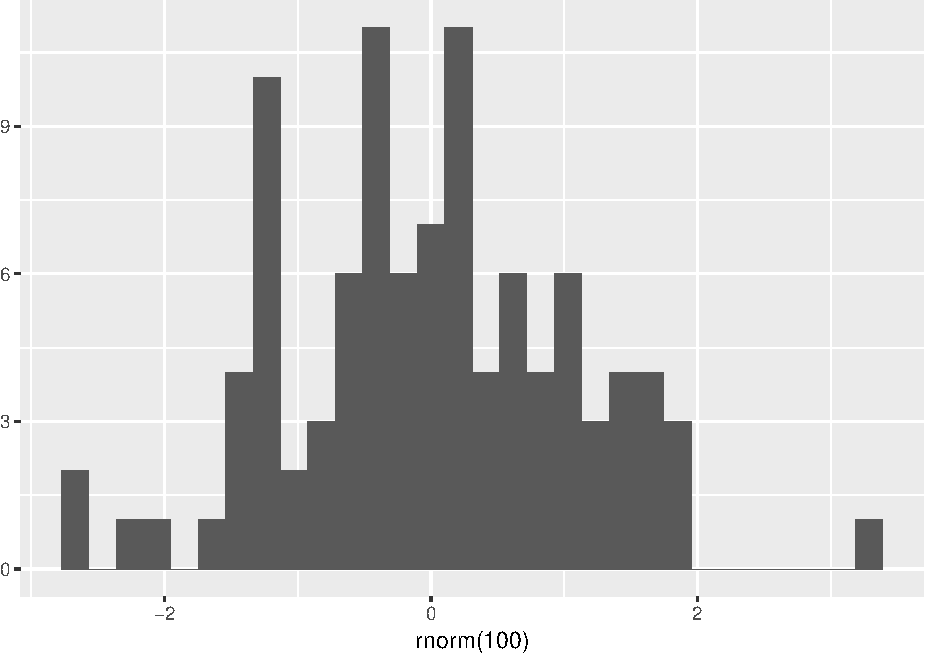
\includegraphics{slow-r_files/figure-latex/unnamed-chunk-52-1.pdf}

This tells R to use the \texttt{qplot()} function from the
\texttt{ggplot2} package to i) generate a random normal set of 100
numbers and ii) plot them.

Try typing \texttt{ggplot2} and pausing or hitting the \texttt{tab} key.
You'll see a pop-up list of functions in the \texttt{ggplot2} package.
Again, this is the best way to call function from a package because it
is unambiguous about what function we want.

An older, alternative way is to load the package into memory using the
\texttt{library()} command. If we enter
\texttt{library(\textquotesingle{}ggplot2\textquotesingle{})} at the
Console, then we can type the simpler expression
\texttt{qplot(rnorm(100))} to create the plot. This seems like less
typing.

So, why do I recommend the other way? Because some packages use the same
names for very similar functions. If you load both into memory, R won't
know which package you want, and so it will choose for you. R will warn
you when it makes this choice saying `function X is masked by package
Y'. Usually, the developers of packages don't create functions with
identical names that do incompatible things, so it's not a huge source
of worry. The problem is magnified when you start to share your code
with other researchers who don't have all of the same packages installed
as you do. So, that's why it's better practice to be specific about the
package(s) you're using when you use particular functions. In fact, CRAN
requires this when you create a package for review.

\subsection{Scripts and functions}\label{scripts-and-functions}

The real power of R, or really any programming language, stems from the
combination of single steps to form more complex and useful wholes. Not
only can we use functions other R experts have provided via packages,
but we can create our own customized sequences of work and save them for
later reuse in the form of scripts and functions.

\subsubsection{Source pane}\label{source-pane}

While it can be fun and instructive to work solely in the Console, for
most real work, you'll want and need to put commands in a place you can
easily reuse them. That place is called the `Source' pane. It's
\texttt{ctrl-1} on your keyboard.

Why is it called source? It's the source of inspiration, the source of
your soon-to-be-realized statistical genius. And the term comes from the
computer world where every project starts out as `source code'.

\subsubsection{Scripts}\label{scripts}

Let's make some source code. Press
\texttt{shift-(command\ or\ control)-n} (that's 3 keys at one time) to
create a new R script file called \texttt{Untitled1}.

Press \texttt{ctrl-1} to make sure that you are typing in the Source
pane in the \texttt{Untitled1} window.

You can type in this window now, but I urge you to get in the habit of
doing two things:

\begin{enumerate}
\def\labelenumi{\arabic{enumi}.}
\tightlist
\item
  Typing in a comment line so you know what's to come.

  \begin{itemize}
  \tightlist
  \item
    Comments require a \texttt{\#} in the first column.
  \item
    So something like \texttt{\#\ R\ Bootcamp\ work\ 2018-08-16} might
    be a good name.
  \item
    Why the weird date format? It's unambiguous across the world, and it
    sorts nicely.
  \end{itemize}
\item
  Saving the file.

  \begin{itemize}
  \tightlist
  \item
    Where to save it and with what name can get very\ldots{}personal.
  \item
    I strongly suggest you start and maintain your own file directory
    structure so that you can find things in the future.
  \item
    My suggestion would be to have a structure like this:

    \begin{itemize}
    \tightlist
    \item
      \texttt{courses/2018\_r\_bootcamp/}
    \end{itemize}
  \item
    And then save the file as \texttt{2018\_08\_16\_script.R} under that
    directory.
  \end{itemize}
\end{enumerate}

Later today, I'm going to sharpen and modify this recommendation
slightly by adding a step that takes advantage of RStudio's project
management functionality. For now, this will be okay.

Now you can type R code and comments in the Source pane. Let's try
something (modestly) useful.

\begin{verbatim}
# Generate data
data_mean_zero <- rnorm(n = 100, mean = 0, sd = 1)
data_mean_nonzero <- rnorm(n = 100, mean = 3, sd = 1)
\end{verbatim}

When you've typed this, press \texttt{(command/control)-s} to save it.

What do these commands do? The \texttt{rnorm()} command creates a random
sample of normally distributed numbers. The \texttt{n}, \texttt{mean},
and \texttt{sd} parameters specify the size of our sample, its mean and
standard deviation. Notice the different sample means.

Now, type in two additional rows of commands.

\begin{verbatim}
# Print histograms
hist(data_mean_zero)
hist(data_mean_nonzero)
\end{verbatim}

Hit \texttt{(command/control)-s} to save.

What is this new \texttt{hist()} command? Let's ask R to tell us. Hit
\texttt{ctrl-2} to go to the Console. Type
\texttt{help(\textquotesingle{}hist\textquotesingle{})} and hit enter.
You can also type \texttt{??hist} to see a broader search of R's help
pages for other commands that start with these letters.

So, this script is going to generate some data and plot histograms.
Let's run the \texttt{hist()} commands. Move up or down arrow into the
line with the \texttt{hist(data\_mean\_zero)} command. Hit the
\texttt{Run} button at the top of the Source panel. \textbf{Notice} that
R moves the highlighted line down by one each time you press the
\texttt{Run} button.

What if you don't want to take your hands off the keyboard to do this?
Good for you! You can run the current line by pressing
\texttt{shift+enter}. Try that.

Now, let's add two more lines to our script.

\begin{verbatim}
# Run t-tests
(t.test(data_mean_zero))
(t.test(data_mean_nonzero))
\end{verbatim}

You can predict what these will do. Confirm it by running the lines.

If you didn't save the file, the name will be highlighted in red. Save
it now.

\subsubsection{\texorpdfstring{`Sourcing' a
script}{Sourcing a script}}\label{sourcing-a-script}

Now that you've saved a sequence of commands, you can run the whole
(saved) sequence from the console. Switch to the console with
\texttt{ctrl-2}.

Enter
\texttt{source(\textquotesingle{}2018\_08\_16\_script.R\textquotesingle{})}
(or whatever name you have given your script) but do not press enter
yet. Let's see what the \texttt{source()} command does. Press
\texttt{esc} to clear the console. Type
\texttt{help(\textquotesingle{}source\textquotesingle{})} to view the
documentation about \texttt{source()}. Now, we know that it will take
the source file we provide and send it to the R console. Make sure
you're still in the console by pressing \texttt{ctrl-2}. Type
\texttt{source(file\ =\ "} and hit \texttt{tab} to see a list of files
in your local directory. If you see the script file you created and
saved, hit return to select it. Then press the right arrow key to the
end of the line, and type \texttt{)} to close the command and
\texttt{enter} to run it.

You may also run the script from the Source panel. Press \texttt{ctrl-1}
to switch to the Source. Press \texttt{ctrl-s} to make sure the file is
saved. Press the \texttt{Source} button in the right corner of the
Source panel.

Why do the plot shapes change each time?

\subsubsection{PaRameteRize your (R)
life}\label{parameterize-your-r-life}

So, this script is fine, but it could be better. What if we want to try
different values for the means or the standard deviations or the number
of samples?

Add this text to the top of your script file.

\begin{verbatim}
# Parameters
mean_1 <- 0
mean_2 <- 3
sd_1 <- 1
sd_2 <- 1
samples_1 <- 100
samples_2 <- 100
\end{verbatim}

Then, edit the next few lines as follows

\begin{verbatim}
(data_mean_zero <- rnorm(n = samples_1, 
                         mean = mean_1, 
                         sd = sd_1))
(data_mean_nonzero <- rnorm(n = samples_2, 
                            mean = mean_2, 
                            sd = sd_2))
\end{verbatim}

See how we've substituted the new parameters for specific values? Save
the script and source it.

If you want to see different plots, switch to the Plots panel
(\texttt{ctrl-6}) and press the left or right arrow buttons.

The virtue of this approach is that we can edit the parameters in the
script and see the effects of the changes pretty quickly. The downside
of this approach is that we still have a lot of duplicate typing.

\subsection{From scripts to functions}\label{from-scripts-to-functions}

Scripts are great. Functions are even better. Functions further reduce
typing and other sorts of errors.

Let's make our own function to see why. It can live (for now) in the
same script file. The basic function will look like this:

\begin{verbatim}
my_hist_t <- function() {}
\end{verbatim}

So, we'll assign the function a name--here \texttt{my\_hist\_t}. Why
this particular name? Well, it's my function, not R's, and it plots a
histogram and runs a \(t\) test. It's boring, but helpful to your future
self to name things in ways that are as clear as possible. Some even
suggest that functions should have verbs in their names --
\texttt{print\_hist\_t()} -- so we can tell them apart from other kinds
of objects.

Our function will have some input parameters--not specified yet--entered
inside the parentheses \texttt{()}. And then there are the squiggly
braces \texttt{\{\}}. Those are new. That's where the meat of the
function goes, the commands we want to execute.

What input parameters will we want to enter? The number of samples,
mean, and standard deviation, of course.

\begin{verbatim}
my_hist_t <- function(my_samples, my_mean, my_sd) {}
\end{verbatim}

Notice that I called the parameters \texttt{my\_samples}, etc. This is
to make it easier to see what's going on inside the function. It's often
good practice to give some default values for the parameters so that
your function runs even if you forget to give it input.

\begin{verbatim}
my_hist_t <- function(my_samples = 100, my_mean = 0, my_sd = 1) {}
\end{verbatim}

If we forget (or choose not) to enter a value for one of the parameters,
our function will use the defaults. Now we type the code.

\begin{Shaded}
\begin{Highlighting}[]
\NormalTok{my_hist_t <-}\StringTok{ }\ControlFlowTok{function}\NormalTok{(}\DataTypeTok{my_samples =} \DecValTok{100}\NormalTok{, }\DataTypeTok{my_mean =} \DecValTok{0}\NormalTok{, }\DataTypeTok{my_sd =} \DecValTok{1}\NormalTok{) \{}
\NormalTok{    my_data <-}\StringTok{ }\KeywordTok{rnorm}\NormalTok{(}\DataTypeTok{n =}\NormalTok{ my_samples, }\DataTypeTok{mean =}\NormalTok{ my_mean, }\DataTypeTok{sd =}\NormalTok{ my_sd)}
    \KeywordTok{hist}\NormalTok{(my_data)}
    \KeywordTok{t.test}\NormalTok{(my_data)}
\NormalTok{\}}
\end{Highlighting}
\end{Shaded}

Let's make sure we understand what's going on. Inside the function
(inside the curly brackets), we compute a random normal data set and
assign it to \texttt{my\_data}. Then we calculate the histogram and
\(t\) test. R will `return' to us the result of the last command in the
function, in this case, the results of \texttt{t.test(my\_data)}.

Let's save the script and source it. We have to do this \textbf{every
time we edit the script file}.

Now switch to the \texttt{Environment} pane (\texttt{ctrl-8}). See how
there is now a function called \texttt{my\_hist\_t} listed? We can now
go back to the console (\texttt{ctrl-2}) and run our function with all
sorts of parameter combinations:

\begin{Shaded}
\begin{Highlighting}[]
\CommentTok{# Run these in the Console}
\KeywordTok{my_hist_t}\NormalTok{()}
\end{Highlighting}
\end{Shaded}

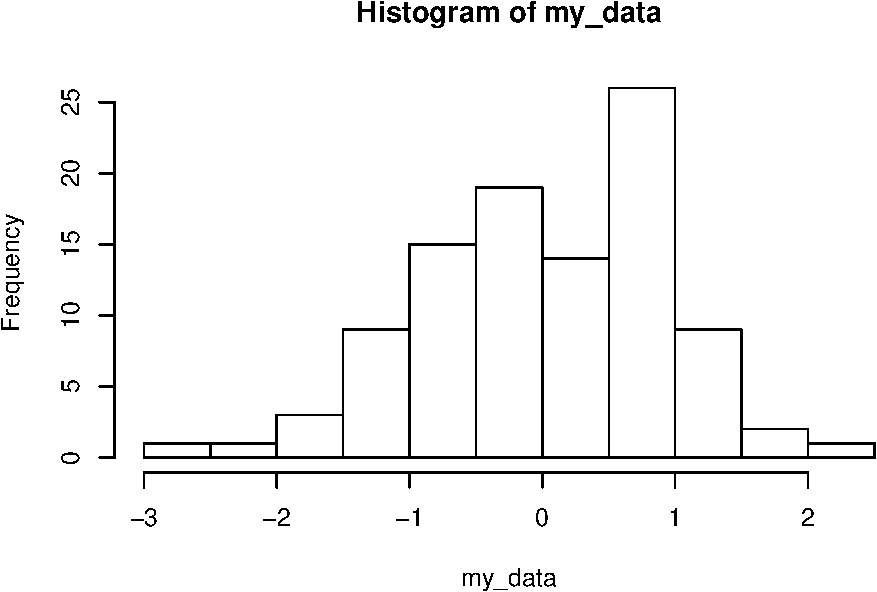
\includegraphics{slow-r_files/figure-latex/unnamed-chunk-54-1.pdf}

\begin{verbatim}
## 
##  One Sample t-test
## 
## data:  my_data
## t = 0.15434, df = 99, p-value = 0.8777
## alternative hypothesis: true mean is not equal to 0
## 95 percent confidence interval:
##  -0.1722467  0.2013031
## sample estimates:
##  mean of x 
## 0.01452816
\end{verbatim}

\begin{Shaded}
\begin{Highlighting}[]
\KeywordTok{my_hist_t}\NormalTok{(}\DataTypeTok{my_mean =} \DecValTok{10}\NormalTok{)}
\end{Highlighting}
\end{Shaded}

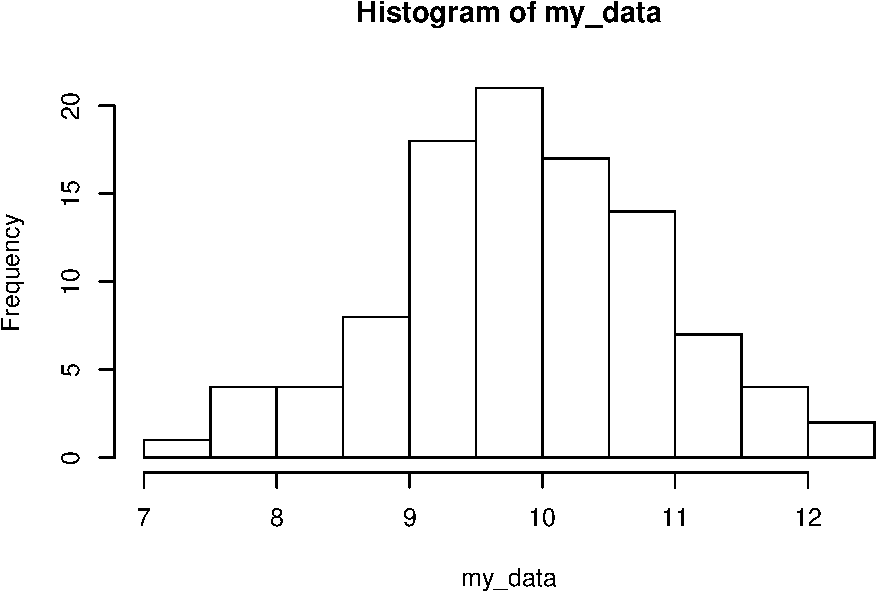
\includegraphics{slow-r_files/figure-latex/unnamed-chunk-54-2.pdf}

\begin{verbatim}
## 
##  One Sample t-test
## 
## data:  my_data
## t = 96.685, df = 99, p-value < 2.2e-16
## alternative hypothesis: true mean is not equal to 0
## 95 percent confidence interval:
##   9.658945 10.063701
## sample estimates:
## mean of x 
##  9.861323
\end{verbatim}

\begin{Shaded}
\begin{Highlighting}[]
\KeywordTok{my_hist_t}\NormalTok{(}\DataTypeTok{my_samples =} \DecValTok{200}\NormalTok{, }\DataTypeTok{my_sd =} \DecValTok{5}\NormalTok{)}
\end{Highlighting}
\end{Shaded}

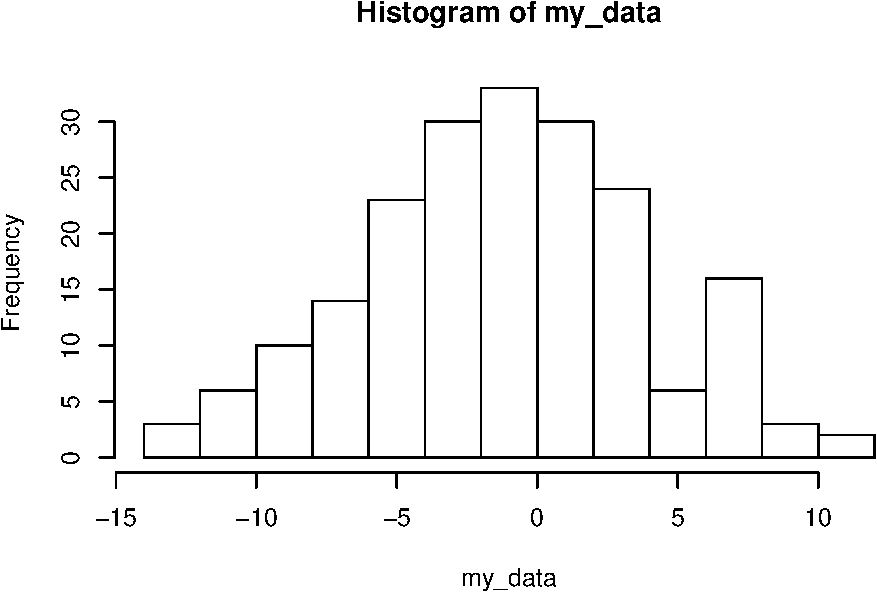
\includegraphics{slow-r_files/figure-latex/unnamed-chunk-54-3.pdf}

\begin{verbatim}
## 
##  One Sample t-test
## 
## data:  my_data
## t = -3.2403, df = 199, p-value = 0.0014
## alternative hypothesis: true mean is not equal to 0
## 95 percent confidence interval:
##  -1.8433850 -0.4485606
## sample estimates:
## mean of x 
## -1.145973
\end{verbatim}

Because we've specified defaults and are naming our parameters when we
call the function, R will just use the defaults when we don't specify a
parameter.

There are many subtleties about writing functions that we haven't
covered here. I recommend the free
\href{http://www.datacamp.com}{DataCamp} course by Hadley Wickham on
\href{https://www.datacamp.com/courses/writing-functions-in-r}{``Writing
Functions in R''} to learn more.

\subsection{Summing up}\label{summing-up-2}

We've learned how to install packages via the
\texttt{install.packages()} command, load packages into R's `working
memory' via \texttt{library()} and to view documentation about packages
using the \texttt{library(help\ =\ "package\_name")} command.

We've also learned how to type sequences of assignments and commands
into the Source pane to create scripts, and we've learned how to execute
those commands using the \texttt{source()} command. We've also seen how
to make a function that encapsulates these sequences into easily
reproducible units, using the
\texttt{function\_name\ \textless{}-\ function(...arguments...)\ \{...function\ commands...\}}
syntax.

There is much more to say and learn about functions (e.g., see this
\href{https://swcarpentry.github.io/r-novice-inflammation/02-func-R/index.html}{Software
Carpentry lesson}), but this is a good start on why they're so important
and useful.

\section{Honing your expertise}\label{honing-your-expertise}

In a short first course in R, we can never cover everything, but we can
hope to give you enough momentum to get started. In this short section,
we'll talk about some skills that will help accelerate your progress in
learning R and RStudio.

\subsection{Practice}\label{practice}

\begin{quote}
The absent-minded maestro was racing up New York's Seventh Avenue to a
rehearsal, when a stranger stopped him. ``Pardon me,'' he said, ``can
you tell me how to get to Carnegie Hall?'' ``Yes,'' answered the maestro
breathlessly. ``Practice!''
\end{quote}

\url{https://quoteinvestigator.com/2010/05/06/how-do-you-get-to-carnegie-hall/}

Using R and RStudio is a skill. To gain expertise, you need to practice.
I recommend practicing at least 3-5 times a week.

\subsection{Use the keyboard}\label{use-the-keyboard}

Train your fingers to limit mousing. Press \texttt{ctrl-2} to switch to
the console. Press \texttt{up\ arrow} to see the recent history of your
console commands. Use the left and right arrow keys to move within/edit
a prior command. Press \texttt{ctrl-a} to go to the beginning of a line
in the console; \texttt{ctrl-e} to go to the end. Type the first few
characters of a variable or command and then i) wait a bit or ii) press
tab to see a list of possible completions. Hit up and down arrows to
scroll through the list. Hit \texttt{enter} to select an item. Hit
\texttt{escape} to clear the current line of the console.

If you want to see a window of your recent commands, go to the
\texttt{History} pane by pressing \texttt{ctrl-4}. You can use the up
and down arrow keys to scroll through your previous commands. Hitting
\texttt{enter} immediately copies that command to the console and
executes it. I find it somewhat less useful than just the up/down arrow
functions in the console, but YMMV.

There will be other keyboard commands. For example, if you're not
already using \texttt{(command/ctrl)+c} for copying,
\texttt{(command/ctrl)+v} for pasting, and \texttt{(command/ctrl)+x} for
cutting, start now. Also, I use \texttt{(command/ctrl)+} (enlarge text)
and \texttt{(command/ctrl)-} (shrink text).

\subsection{Reading code will improve your
writing}\label{reading-code-will-improve-your-writing}

It's well known that the best writers of prose, poetry, or music, are
often voracious consumers. The more comfortable you get reading others'
code, the better your own writing will become. Yes, code can be dense at
times, and some coders write cleaner and more comprehensible code than
others. But in this workshop, we're trying to help speed you along the
learning curve by helping you learn to read R code from the get-go.
Remember, it's critically important that code be human-readable.
Computers want 1's and 0's and don't really care about things like
comments or elegant syntax or any of that.

\subsection{Getting help}\label{getting-help}

Press \texttt{ctrl-3} to go to the help pane.
\href{http://rstudio.com}{RStudio} has extensive documentation and help
resources. Google is your friend, at least in this regard.. There is
also an active R community on \href{http://stackoverflow.com}{Stack
Overflow}.

I often find it useful to read the documentation about a function to see
what the other parameters do. For example, typing
\texttt{help(\textquotesingle{}plot\textquotesingle{})} shows us that
the \texttt{plot()} function takes (typically) two inputs, \texttt{x},
and \texttt{y}. The ellipsis \texttt{...} says that it also takes other
optional parameters. So, this code

\begin{Shaded}
\begin{Highlighting}[]
\KeywordTok{plot}\NormalTok{(}\DataTypeTok{x =} \KeywordTok{rnorm}\NormalTok{(}\DecValTok{10}\NormalTok{), }\DataTypeTok{y =} \KeywordTok{rnorm}\NormalTok{(}\DecValTok{10}\NormalTok{), }\DataTypeTok{main =} \StringTok{"Random scatterplot"}\NormalTok{, }\DataTypeTok{ylab =} \StringTok{"Random Y"}\NormalTok{, }
    \DataTypeTok{xlab =} \StringTok{"Random X"}\NormalTok{)}
\end{Highlighting}
\end{Shaded}

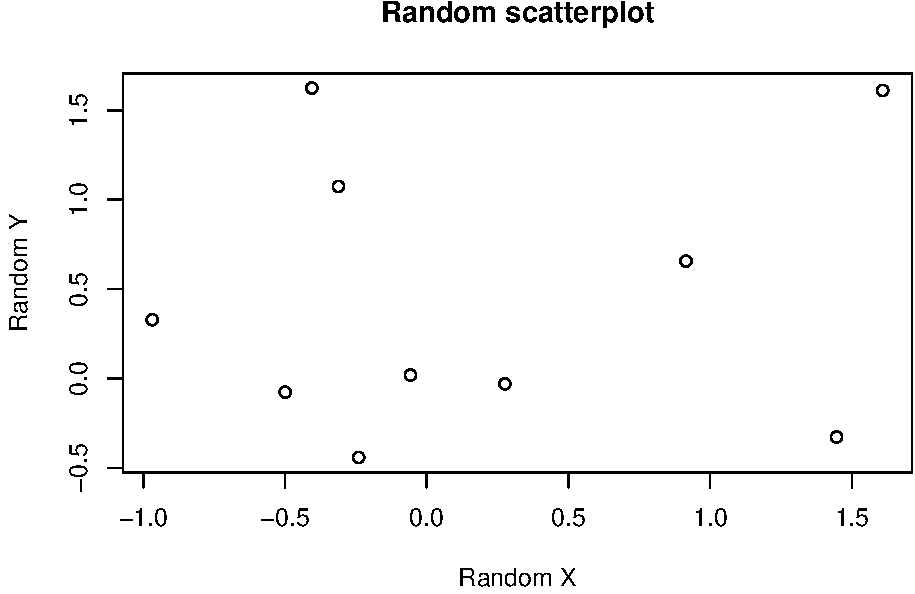
\includegraphics{slow-r_files/figure-latex/unnamed-chunk-55-1.pdf}

Creates a scatter plot with a title and labels for the x and y axes.

\subsection{Control/view the local
environment}\label{controlview-the-local-environment}

You'll want to practice `situational awareness'. That means knowing
what's going on in your local R environment.

Press \texttt{ctrl-8} to go to the `Environment' pane. This shows us all
of the Data, Variables, and Functions we have defined in the current
session. Some of the items can be expanded by clicking on the small
arrow, the data frame for example.

\subsubsection{What's assigned to what}\label{whats-assigned-to-what}

The Environment pane is one way to keep track of what you've assigned,
but there are some other ways to do this from the console.

\begin{itemize}
\tightlist
\item
  The `list objects' command or \texttt{ls()} tells you what objects and
  functions are in R's active memory ready for your use.
\item
  Typing an object's name at the console and hitting \texttt{enter} will
  give you the current value.
\end{itemize}

If you're exploring and putting your commands in a script, you may find
it useful to `clean the slate' or start with a fresh environment before
you \texttt{source()} your script. To do this, you can `remove
individual objects' using the \texttt{rm()} command, or remove all of
them using \texttt{rm(list\ =\ ls())}.

\subsection{Finding your way around}\label{finding-your-way-around}

We've mostly ignored it thus far, but when you start RStudio, all of
your work is in a default directory (or folder) on your computer. You
can change this default in the `Tools' menu, `Global Options\ldots{}'
item. Later this afternoon, I'm going to recommend that you let RStudio
help you organize your work by creating a project with its own directory
for each new project you take on. But for now, let's see how we can use
console commands to find out where we are.

\subsubsection{Working directories and
navigation}\label{working-directories-and-navigation}

To find out what directory you're currently working in, type the get
working directory command \texttt{getwd()} at the console.

\begin{Shaded}
\begin{Highlighting}[]
\KeywordTok{getwd}\NormalTok{()}
\end{Highlighting}
\end{Shaded}

\begin{verbatim}
## [1] "/Users/rick/github/psu-psychology/r-bootcamp-2018/talks"
\end{verbatim}

You'll see that I have a directory hierarchy under my home
(\texttt{rick/}) directory that is specifically devoted to GitHub
projects, with a subdirectory for the \texttt{psu-psychology} repository
on GitHub and then this specific bootcamp project.

I can go `up' the directory hierarchy by typing the set working
directory command \texttt{setwd()} as follows:

\begin{verbatim}
setwd("../") # "../" means go up one level in the directory hierarchy
getwd()
\end{verbatim}

To go back to where I was, I have to enter the name of the old directory
where I came from. If I remember it, I just enter the \texttt{setwd()}
command again.

\begin{verbatim}
setwd("r-bootcamp-2018/")
\end{verbatim}

But if I've forgotten, RStudio can help me. Type the start of the
\texttt{setwd(\textquotesingle{}} command and then pause or hit the
\texttt{tab} key. RStudio will show you a list of the contents of the
current working directory. Use the up or down arrow keys to select where
you want to change to, and then press \texttt{enter}. Confirm that you
are where you thought you wanted to be with \texttt{getwd()}.

Some researchers have workflows where they set the working directory in
their scripts (using \texttt{setwd()}), but \textbf{these workflows are
often more likely to break when they are shared with other people}.
Nevertheless, you will need to have a mental model of the directory
hierarchy you've created for your work and be explicit about where you
want data, scripts, and outputs to go. This is critical when you start
writing scripts and functions, and you want to tell your script or
function where to find its inputs, like the data files you'll want to
process.

For example, if my R scripts are stored in an \texttt{R/} directory
under my working directory as indicated below, to \texttt{source()}
them, I need to give a command like this
\texttt{source(\textquotesingle{}R/my\_script.R)}. And if my data are
stored in a \texttt{data/csv/} directory, I may have to give my data
cleaning function an input like this:
\texttt{clean\_my\_data(path\_to\_data\ =\ \textquotesingle{}data/csv/dirty\_data.csv\textquotesingle{})}

So, what directory structure should you use?

\subsubsection{Directory structures}\label{directory-structures}

One of the reasons people gravitate toward careers in independent
research is that they relish their independence. So, you'll find lots of
advice about how to structure the information in your projects. Rather
than tell you what structure to use, I'm going to show you some
structures that I find sensible and workable for many research projects:

\begin{verbatim}
my_awesome_project/
  README.md
  data/
    raw/
      sub_001.xlsx # or ...
      sub_002.xlsx
    csv/
      sub_001.csv
      sub_002.csv
    aggregate/
  R/ # Helper scripts
  figs/
  pubs/
    papers/
    talks/
    posters/
\end{verbatim}

This means that the \texttt{my\_awesome\_project/} directory is the
`home' directory for this project.

Some people prefer to organize their data by measure:

\begin{verbatim}
my_awesome_project/
  README.md
  data/
    behavior/
    mri_structural/
    mri_functional/
...
\end{verbatim}

And others prefer to organize it by participant:

\begin{verbatim}
my_awesome_project/
  README.md
  data/
    sub_001/
      sub_001_behavior.csv
      sub_001_mri_structural/
      sub_002_mri_functional/
...
\end{verbatim}

\begin{quote}
Choose a directory structure that works for you and try to be as
consistent as possible about it. This will make writing reproducible
scripts (within and across projects) much easier.
\end{quote}

By the way, you can automate the creation of directories using the
\texttt{dir.create()} command, but I usually use the RStudio Files panel
and its associated buttons.

\subsection{Configuring RStudio}\label{configuring-rstudio}

You can customize your RStudio environment to your heart's content,
including rearranging how the different panels appear. Go for it. You
can modify the settings using the `Tools' menu `Project Options' item.
The Project Options window opens. Here's mine.

I have strong feelings about two settings:

\begin{itemize}
\tightlist
\item
  \texttt{Restore\ .RData\ into\ workspace\ at\ startup} should be
  \textbf{unchecked}.
\item
  \texttt{Save\ workspace\ to\ .RData\ on\ exit} should be
  \textbf{\texttt{never}}.
\end{itemize}

These settings ensure that you have a `clean' R session when you
start-up. That is, that old values of variables and functions aren't
still lurking about. This may seem counter-intuitive, but it is
considered a best practice for reproducible research. You'll want to be
able to re-generate your results from scratch without having old (stale,
possibly outdated) values interfering with your current analyses.

\section{Getting data in}\label{getting-data-in}

There are three main sources of data: R packages, the internet, and
files on local computers or servers you have access to.

\subsection{Data from R packages}\label{data-from-r-packages}

Base R comes with a number of datasets that can be good for learning
your way around. Type \texttt{library(help="datasets")} to see a list of
them.

\begin{Shaded}
\begin{Highlighting}[]
\KeywordTok{library}\NormalTok{(}\DataTypeTok{help =} \StringTok{"datasets"}\NormalTok{)}
\end{Highlighting}
\end{Shaded}

Type \texttt{help(\textquotesingle{}mtcars\textquotesingle{})} for
information about the Motor Trend cars dataset, for example. Type
\texttt{data(\textquotesingle{}mtcars\textquotesingle{})} to load that
dataset into memory.

\subsection{Data from the internet}\label{data-from-the-internet}

There is a lot of publicly available data on the internet. But each
dataset and site has its own way of downloading.

Just to illustrate how this might work, try downloading a simple heart
rate timeseries using the \texttt{read.csv()} command:

\begin{Shaded}
\begin{Highlighting}[]
\NormalTok{hr_mit <-}\StringTok{ }\KeywordTok{read.csv}\NormalTok{(}\DataTypeTok{file =} \StringTok{"http://ecg.mit.edu/time-series/hr.11839"}\NormalTok{, }\DataTypeTok{header =} \OtherTok{FALSE}\NormalTok{, }
    \DataTypeTok{col.names =} \StringTok{"HR"}\NormalTok{, }\DataTypeTok{skip =} \DecValTok{0}\NormalTok{)}
\end{Highlighting}
\end{Shaded}

The \texttt{read.csv()} command creates a data frame. Note that we
specified a URL or web address for the file and some other parameters.
This file has no header with the column names, so we said
\texttt{header\ =\ FALSE}; we provided a name for the single column
\texttt{col.names\ =\ \textquotesingle{}HR\textquotesingle{}}; and we
said not to skip any rows at the top of the file \texttt{skip\ =\ 0}.

\begin{Shaded}
\begin{Highlighting}[]
\KeywordTok{class}\NormalTok{(hr_mit)}
\end{Highlighting}
\end{Shaded}

\begin{verbatim}
## [1] "data.frame"
\end{verbatim}

Note that we don't have to surround `hr\_mit' with quotation marks
because it is a name that R should know because we just defined it.

Then we can plot it using \texttt{plot(hr\_mit\$HR)}

\begin{Shaded}
\begin{Highlighting}[]
\KeywordTok{plot}\NormalTok{(hr_mit}\OperatorTok{$}\NormalTok{HR)}
\end{Highlighting}
\end{Shaded}

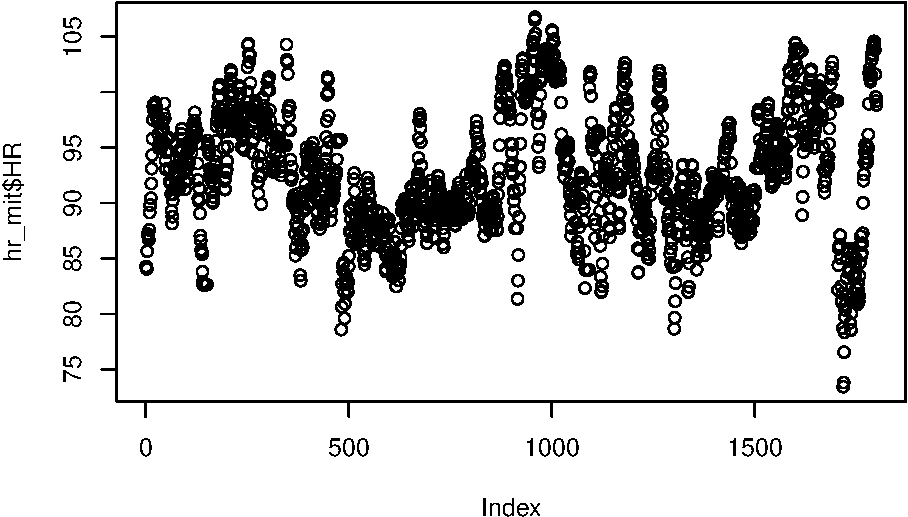
\includegraphics{slow-r_files/figure-latex/unnamed-chunk-60-1.pdf}

\subsubsection{Public data from the Open Science Framework
(OSF)}\label{public-data-from-the-open-science-framework-osf}

Samuel Mehr et al. (2018) have provided some data files using the Open
Science Framework:

Mehr, S. A., Singh, M., York, H., Glowacki, L., \& Krasnow, M. (2018,
January 9) Datasets. \url{https://doi.org/10.17605/OSF.IO/M9RXV}

Let's download the survey data.

\begin{Shaded}
\begin{Highlighting}[]
\NormalTok{mehr_etal_survey <-}\StringTok{ }\KeywordTok{read.csv}\NormalTok{(}\DataTypeTok{file =} \StringTok{"https://osf.io/etg8z/download"}\NormalTok{)}
\KeywordTok{names}\NormalTok{(mehr_etal_survey)}
\end{Highlighting}
\end{Shaded}

\begin{verbatim}
## [1] "ethno"  "theory" "musoth" "psych"  "tenure" "sex"    "age"    "naiv1" 
## [9] "naiv2"
\end{verbatim}

This will produce a cross tabulated table about the sex and tenure
status of the respondents:

\begin{Shaded}
\begin{Highlighting}[]
\KeywordTok{xtabs}\NormalTok{(}\DataTypeTok{formula =} \OperatorTok{~}\NormalTok{sex }\OperatorTok{+}\StringTok{ }\NormalTok{tenure, }\DataTypeTok{data =}\NormalTok{ mehr_etal_survey)}
\end{Highlighting}
\end{Shaded}

\begin{verbatim}
##                         tenure
## sex                        0   1
##   Female                 203 187
##   I prefer not to answer  46  62
##   Male                   150 289
##   Other                    2   1
\end{verbatim}

Here is the same table formatted in a nice way using the
\texttt{knitr::kable()} function:

\begin{Shaded}
\begin{Highlighting}[]
\NormalTok{knitr}\OperatorTok{::}\KeywordTok{kable}\NormalTok{(}\KeywordTok{xtabs}\NormalTok{(}\DataTypeTok{formula =} \OperatorTok{~}\NormalTok{sex }\OperatorTok{+}\StringTok{ }\NormalTok{tenure, }\DataTypeTok{data =}\NormalTok{ mehr_etal_survey))}
\end{Highlighting}
\end{Shaded}

\begin{longtable}[]{@{}lrr@{}}
\toprule
& 0 & 1\tabularnewline
\midrule
\endhead
Female & 203 & 187\tabularnewline
I prefer not to answer & 46 & 62\tabularnewline
Male & 150 & 289\tabularnewline
Other & 2 & 1\tabularnewline
\bottomrule
\end{longtable}

\subsection{An aside about comma-separated value (CSV)
files}\label{an-aside-about-comma-separated-value-csv-files}

Spreadsheets are incredibly powerful computational tools. But they are
terrible ways of storing data you want to use in R.

Imagine a future for yourself where you rarely do any manipulation or
visualization of data using a spreadsheet. Work to realize that future
as soon as possible.

Why? Because you want to produce open, transparent, and reproducible
scientific workflows using data and processing pipelines that are
findable, accessible, interoperable, and reusable (FAIR) \footnote{Wilkinson,
  M. D., Dumontier, M., Aalbersberg, I. J. J., Appleton, G., Axton, M.,
  Baak, A., Blomberg, N., et al. (2016). The FAIR guiding principles for
  scientific data management and stewardship. \emph{Scientific Data},
  \emph{3}, 160018. Retrieved from
  \url{http://dx.doi.org/10.1038/sdata.2016.18}}.

Comma-separated value (CSV) files are text files with items separated by
commas, and rows separated by new line or return characters. CSV files
have the file extension \texttt{.csv}. All spreadsheet programs can
export and import CSV files.

CSV files are the \emph{lingua franca} of the data science world,
followed closely by tab-delimited files (where \texttt{tab} characters
replace the commas), JavaScript Object Notation (JSON), and eXtensible
Markup Language (XML). Here is a tutorial about CSV files:
\url{https://swcarpentry.github.io/r-novice-inflammation/11-supp-read-write-csv/}

\subsubsection{\texorpdfstring{Reading `foreign' file
formats}{Reading foreign file formats}}\label{reading-foreign-file-formats}

Notwithstanding the fact that we urge you to store data in
comma-separated text files, you will often want and need to work with
data files stored in other formats.

The `foreign' package
(\texttt{install.packages(\textquotesingle{}foreign\textquotesingle{})})
contains commands to read SPSS files (\texttt{foreign::read.spss()}),
Stata files (\texttt{foreign::read.dta()}), Systat files
(\texttt{foreign::read.systat()}), and Minitab files
(\texttt{foreign::read.mtp()}).

SAS files can be imported using the \texttt{sas7bdat} package
(\texttt{install.packages(\textquotesingle{}sas7bdat\textquotesingle{})}).

The \texttt{xlsx} package
(\texttt{install.packages(\textquotesingle{}xlsx\textquotesingle{})})
contains commands to read MS Excel (.xlsx) spreadsheets.

These functions all operate to create an R data frame.

\subsection{Local data}\label{local-data}

Much or most of the time, you'll want to load data into R that is stored
on your computer or on a server you have access to.

\begin{quote}
It is a best practice to read-in your data file each time you return to
work on your project.
\end{quote}

\subsection{Exploring data}\label{exploring-data}

Once we have loaded a dataset, we can poke around. We'll use the
\texttt{mtcars} dataset since it's part of base R.

\begin{Shaded}
\begin{Highlighting}[]
\KeywordTok{data}\NormalTok{(mtcars)}
\KeywordTok{class}\NormalTok{(mtcars)}
\end{Highlighting}
\end{Shaded}

\begin{verbatim}
## [1] "data.frame"
\end{verbatim}

\begin{Shaded}
\begin{Highlighting}[]
\KeywordTok{str}\NormalTok{(mtcars)  }\CommentTok{# What is the structure of mtcars?}
\end{Highlighting}
\end{Shaded}

\begin{verbatim}
## 'data.frame':    32 obs. of  11 variables:
##  $ mpg : num  21 21 22.8 21.4 18.7 18.1 14.3 24.4 22.8 19.2 ...
##  $ cyl : num  6 6 4 6 8 6 8 4 4 6 ...
##  $ disp: num  160 160 108 258 360 ...
##  $ hp  : num  110 110 93 110 175 105 245 62 95 123 ...
##  $ drat: num  3.9 3.9 3.85 3.08 3.15 2.76 3.21 3.69 3.92 3.92 ...
##  $ wt  : num  2.62 2.88 2.32 3.21 3.44 ...
##  $ qsec: num  16.5 17 18.6 19.4 17 ...
##  $ vs  : num  0 0 1 1 0 1 0 1 1 1 ...
##  $ am  : num  1 1 1 0 0 0 0 0 0 0 ...
##  $ gear: num  4 4 4 3 3 3 3 4 4 4 ...
##  $ carb: num  4 4 1 1 2 1 4 2 2 4 ...
\end{verbatim}

\begin{Shaded}
\begin{Highlighting}[]
\KeywordTok{names}\NormalTok{(mtcars)}
\end{Highlighting}
\end{Shaded}

\begin{verbatim}
##  [1] "mpg"  "cyl"  "disp" "hp"   "drat" "wt"   "qsec" "vs"   "am"   "gear"
## [11] "carb"
\end{verbatim}

These commands load the dataset, show that it's a data frame, and show
us the names of the columns or variables. We can look at the top (head)
and bottom (tail) of the dataset.

\begin{Shaded}
\begin{Highlighting}[]
\KeywordTok{head}\NormalTok{(mtcars)  }\CommentTok{# display first 6 cases}
\end{Highlighting}
\end{Shaded}

\begin{verbatim}
##                    mpg cyl disp  hp drat    wt  qsec vs am gear carb
## Mazda RX4         21.0   6  160 110 3.90 2.620 16.46  0  1    4    4
## Mazda RX4 Wag     21.0   6  160 110 3.90 2.875 17.02  0  1    4    4
## Datsun 710        22.8   4  108  93 3.85 2.320 18.61  1  1    4    1
## Hornet 4 Drive    21.4   6  258 110 3.08 3.215 19.44  1  0    3    1
## Hornet Sportabout 18.7   8  360 175 3.15 3.440 17.02  0  0    3    2
## Valiant           18.1   6  225 105 2.76 3.460 20.22  1  0    3    1
\end{verbatim}

\begin{Shaded}
\begin{Highlighting}[]
\KeywordTok{tail}\NormalTok{(mtcars)  }\CommentTok{# display last 6 cases}
\end{Highlighting}
\end{Shaded}

\begin{verbatim}
##                 mpg cyl  disp  hp drat    wt qsec vs am gear carb
## Porsche 914-2  26.0   4 120.3  91 4.43 2.140 16.7  0  1    5    2
## Lotus Europa   30.4   4  95.1 113 3.77 1.513 16.9  1  1    5    2
## Ford Pantera L 15.8   8 351.0 264 4.22 3.170 14.5  0  1    5    4
## Ferrari Dino   19.7   6 145.0 175 3.62 2.770 15.5  0  1    5    6
## Maserati Bora  15.0   8 301.0 335 3.54 3.570 14.6  0  1    5    8
## Volvo 142E     21.4   4 121.0 109 4.11 2.780 18.6  1  1    4    2
\end{verbatim}

We can also summarize the data with the \texttt{summary()} command.

\begin{Shaded}
\begin{Highlighting}[]
\KeywordTok{summary}\NormalTok{(mtcars)}
\end{Highlighting}
\end{Shaded}

\begin{verbatim}
##       mpg             cyl             disp             hp       
##  Min.   :10.40   Min.   :4.000   Min.   : 71.1   Min.   : 52.0  
##  1st Qu.:15.43   1st Qu.:4.000   1st Qu.:120.8   1st Qu.: 96.5  
##  Median :19.20   Median :6.000   Median :196.3   Median :123.0  
##  Mean   :20.09   Mean   :6.188   Mean   :230.7   Mean   :146.7  
##  3rd Qu.:22.80   3rd Qu.:8.000   3rd Qu.:326.0   3rd Qu.:180.0  
##  Max.   :33.90   Max.   :8.000   Max.   :472.0   Max.   :335.0  
##       drat             wt             qsec             vs        
##  Min.   :2.760   Min.   :1.513   Min.   :14.50   Min.   :0.0000  
##  1st Qu.:3.080   1st Qu.:2.581   1st Qu.:16.89   1st Qu.:0.0000  
##  Median :3.695   Median :3.325   Median :17.71   Median :0.0000  
##  Mean   :3.597   Mean   :3.217   Mean   :17.85   Mean   :0.4375  
##  3rd Qu.:3.920   3rd Qu.:3.610   3rd Qu.:18.90   3rd Qu.:1.0000  
##  Max.   :4.930   Max.   :5.424   Max.   :22.90   Max.   :1.0000  
##        am              gear            carb      
##  Min.   :0.0000   Min.   :3.000   Min.   :1.000  
##  1st Qu.:0.0000   1st Qu.:3.000   1st Qu.:2.000  
##  Median :0.0000   Median :4.000   Median :2.000  
##  Mean   :0.4062   Mean   :3.688   Mean   :2.812  
##  3rd Qu.:1.0000   3rd Qu.:4.000   3rd Qu.:4.000  
##  Max.   :1.0000   Max.   :5.000   Max.   :8.000
\end{verbatim}

And, we can even plot all of the data.

\begin{Shaded}
\begin{Highlighting}[]
\KeywordTok{plot}\NormalTok{(mtcars)}
\end{Highlighting}
\end{Shaded}

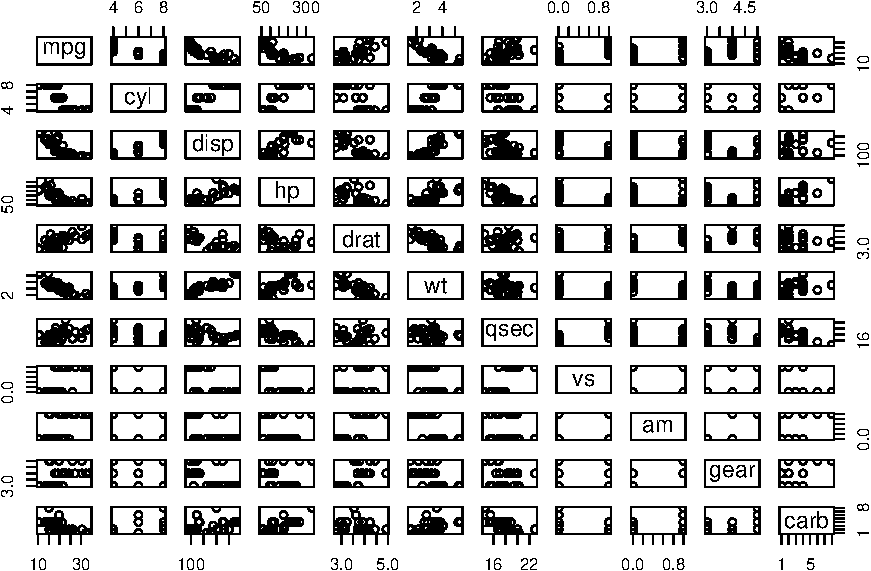
\includegraphics{slow-r_files/figure-latex/unnamed-chunk-67-1.pdf}

We can choose specific subsets of variables like before, and even
customize the way the histogram looks:

\begin{Shaded}
\begin{Highlighting}[]
\NormalTok{guzzlers <-}\StringTok{ }\NormalTok{mtcars}\OperatorTok{$}\NormalTok{mpg }\OperatorTok{<}\StringTok{ }\DecValTok{20}
\KeywordTok{hist}\NormalTok{(mtcars}\OperatorTok{$}\NormalTok{mpg[guzzlers], }\DataTypeTok{main =} \StringTok{"Gas Guzzling Cars in the mtcars dataset"}\NormalTok{, }
    \DataTypeTok{xlab =} \StringTok{"Miles Per Gallon (mpg)"}\NormalTok{)}
\end{Highlighting}
\end{Shaded}

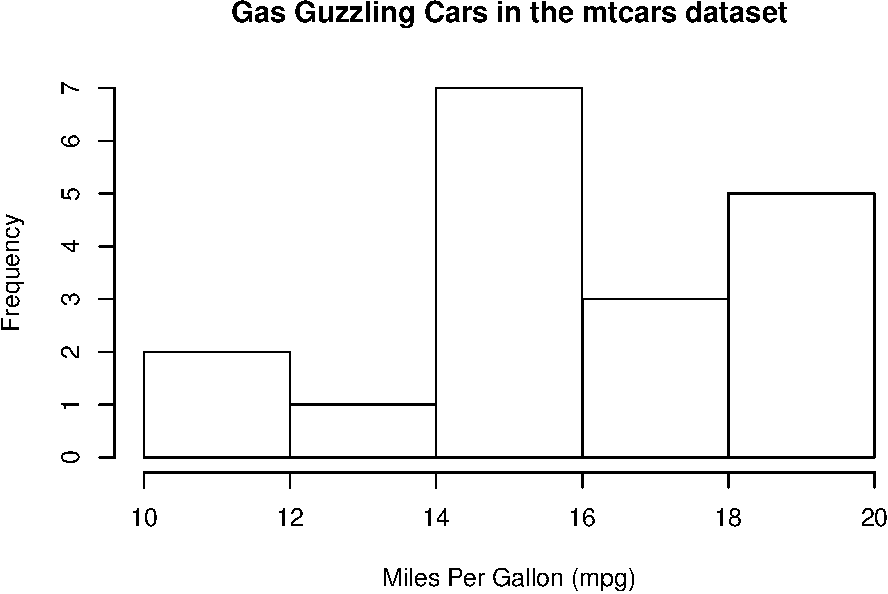
\includegraphics{slow-r_files/figure-latex/unnamed-chunk-68-1.pdf}

\subsection{Summing up}\label{summing-up-3}

\begin{itemize}
\tightlist
\item
  Use \texttt{read.csv()} to read comma-separated value text files
\item
  Use other commands as needed
\item
  Goal is to import a data frame

  \begin{itemize}
  \tightlist
  \item
    \texttt{str()} to show structure of data frame
  \item
    \texttt{names()} to show column names
  \item
    \texttt{summary()} produces summary statistics
  \item
    \texttt{plot()} creates a matrix of plots, pitting each variable
    against the other
  \end{itemize}
\end{itemize}

\section{Materials}\label{materials}

This document was produced on 2018-08-14 08:38:24 in
\href{http://rstudio.com}{RStudio} version 1.1.453 using R Markdown. The
code and materials used to generate the slides may be found at
\url{https://github.com/psu-psychology/r-bootcamp-2018/}. Information
about the R Session that produced the slides is as follows:

\begin{Shaded}
\begin{Highlighting}[]
\KeywordTok{sessionInfo}\NormalTok{()}
\end{Highlighting}
\end{Shaded}

\begin{verbatim}
## R version 3.5.1 (2018-07-02)
## Platform: x86_64-apple-darwin15.6.0 (64-bit)
## Running under: macOS Sierra 10.12.6
## 
## Matrix products: default
## BLAS: /System/Library/Frameworks/Accelerate.framework/Versions/A/Frameworks/vecLib.framework/Versions/A/libBLAS.dylib
## LAPACK: /Library/Frameworks/R.framework/Versions/3.5/Resources/lib/libRlapack.dylib
## 
## locale:
## [1] en_US.UTF-8/en_US.UTF-8/en_US.UTF-8/C/en_US.UTF-8/en_US.UTF-8
## 
## attached base packages:
## [1] stats     graphics  grDevices utils     datasets  methods   base     
## 
## other attached packages:
## [1] tufte_0.4
## 
## loaded via a namespace (and not attached):
##  [1] Rcpp_0.12.18     highr_0.7        pillar_1.3.0     compiler_3.5.1  
##  [5] formatR_1.5      plyr_1.8.4       bindr_0.1.1      base64enc_0.1-3 
##  [9] tools_3.5.1      digest_0.6.15    jsonlite_1.5     evaluate_0.11   
## [13] tibble_1.4.2     gtable_0.2.0     pkgconfig_2.0.1  rlang_0.2.1     
## [17] rstudioapi_0.7   yaml_2.1.19      xfun_0.3         bindrcpp_0.2.2  
## [21] stringr_1.3.1    dplyr_0.7.6      knitr_1.20       rprojroot_1.3-2 
## [25] grid_3.5.1       tidyselect_0.2.4 glue_1.3.0       R6_2.2.2        
## [29] rmarkdown_1.10   ggplot2_3.0.0    purrr_0.2.5      magrittr_1.5    
## [33] backports_1.1.2  scales_0.5.0     codetools_0.2-15 htmltools_0.3.6 
## [37] assertthat_0.2.0 colorspace_1.3-2 labeling_0.3     tinytex_0.6     
## [41] stringi_1.2.4    lazyeval_0.2.1   munsell_0.5.0    crayon_1.3.4
\end{verbatim}

\subsection{Notes}\label{notes}


\end{document}
